\documentclass[a4paper,kulak]{kulakarticle}

\usepackage[utf8]{inputenc}
\usepackage[dutch]{babel}
\usepackage{pdfpages}
\usepackage{subfig}
\usepackage{float}

\usepackage{cite}

% style
%\usepackage[left=2.5cm,top=2cm,right=2.5cm,bottom=2cm,a4paper]{geometry}
\usepackage{color}

\date{\today}
\address{
	Bachelor in de fysica\\
	Bachelor in de informatica\\
	Bachelor in de wiskunde\\
	Ingenieurswetenschappen}
\title{BDA App}
\author{Marthe B\"{o}ting,	Robin Bruneel en Toon Ingelaere}

\begin{document}
	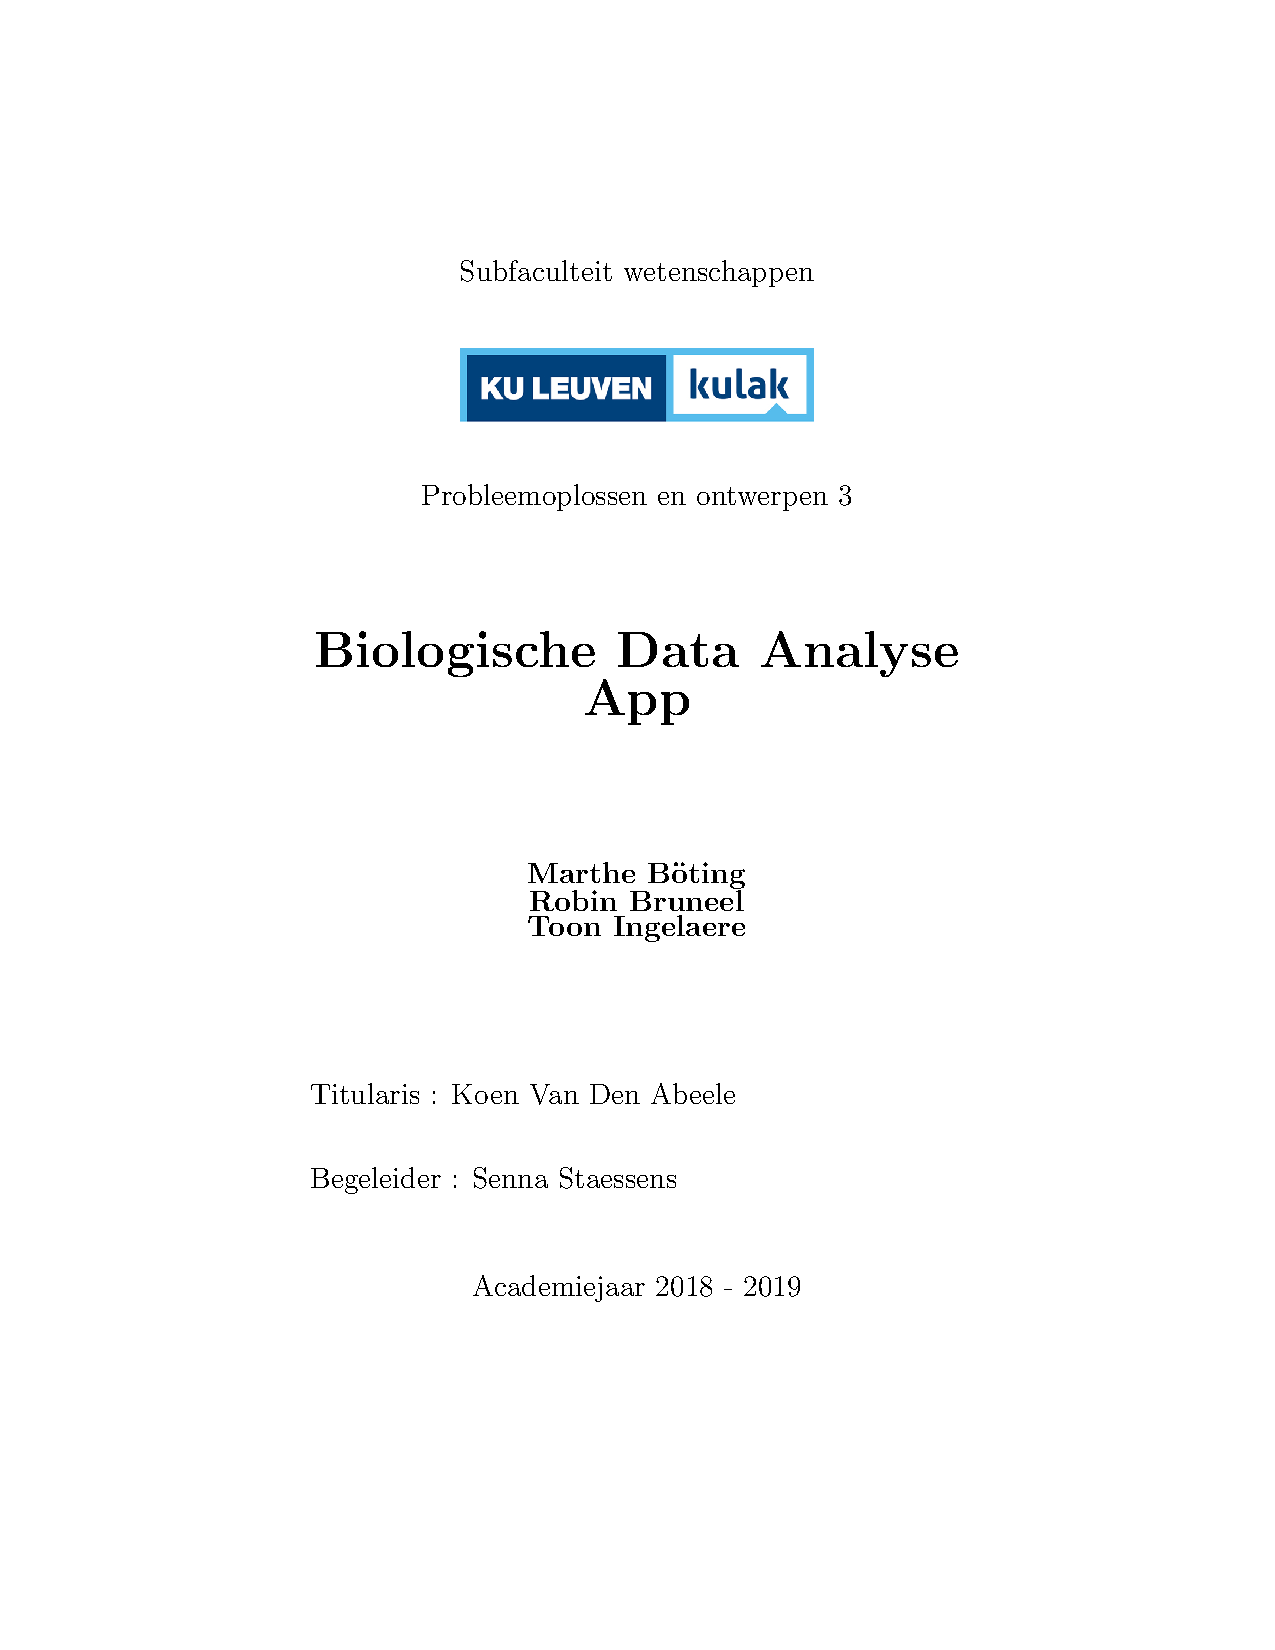
\includepdf{voorblad}
	
	\maketitle

\section*{Inleiding}
Beroertes zijn in de hedendaagse Westerse samenleving de derde grootste doodsoorzaak na hartinfarcten en kanker. Zoals we zien op Figuur \ref{figuur doodsoorzaken} kapen ze op wereldvlak zelfs de tweede plaats weg\cite{worldhealthorganization}. In België komen er gemiddeld 25 000 beroertes per jaar voor. In 15\% van deze gevallen overlijdt de patiënt. De overige 85\% heeft na een beroerte vaak last van blijvende functiebeperkingen zoals cognitieve, emotionele of gedragsproblemen. Een ischemische beroerte ontstaat wanneer een bloedklonter emboliseert en in één van de hersenbloedvaten vast komt te zitten. Deze bloedklonter moet verwijderd worden of de patiënt loopt hersenschade op.
Daarom focust de huidige therapie vooral op het snel en efficiënt verwijderen van de bloedklonter. In eerste instantie kan dit via het geneesmiddel, weefsel plasminogeen activator, proberen de klonter op te lossen. Dit geneesmiddel moet echter gegeven worden binnen 4,5 uur na het optreden van de symptomen. Wanneer men dit geneesmiddel te laat toedient, kan dit leiden tot bloedingen of toxiciteit in de hersenen. Van alle patiënten die het geneesmiddel toegediend krijgen, lost de klonter slechts in 1/3 van de gevallen op. Waardoor men gebruik moet maken van trombectomie om de klonter er manueel uit te halen.\\
Om huidige therapeutische opties te verbeteren en het aantal slachtoffers aan beroertes te doen slinken, gebruikt men deze bloedklonters voor verder onderzoek. Bij dit soort onderzoek probeert men de samenstelling van deze bloedklonters te analyseren. Hiervoor worden afbeeldingen gemaakt van bloedklonter die voor welbepaalde componenten gekleurd zijn zoals bijvoorbeeld rode bloedcellen, witte bloedcellen en bloedplaatjes. Vervolgens wordt de klonter geanalyseerd via kleur-gebaseerde segmentatieanalyse. 
Het manueel analyseren van de bloedklonters is echter erg tijdrovend. Er is ons dan ook gevraagd om een gebruiksvriendelijke app te ontwikkelen die net deze analyse van de afbeeldingen kan automatiseren.
In dit verslag gaan we eerst in op wat de klant specifiek van ons verwacht en aan welke specificaties het ontwerp moet voldoen. Daarna bespreken we het design en lichten we het ook toe. Ten slotte wordt er nog een blik geworpen naar de vakken uit de eerste drie semesters die ons hierbij geholpen hebben.

	\begin{figure}[H]
		\centering
		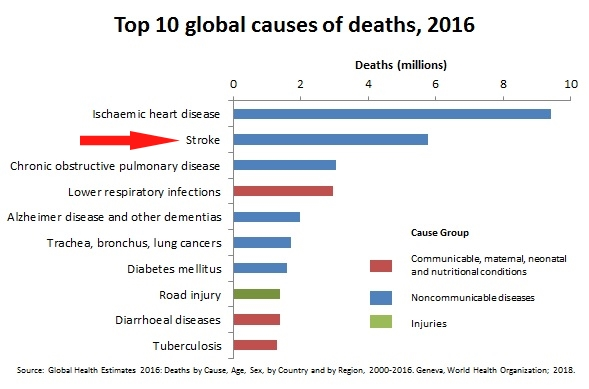
\includegraphics[width = 0.7\textwidth]{top10doodsoorzaken.png}
	
		\caption{Statistieken van de \textit{World Health Organization} van 2016 waarin te zien is dat wereldwijd beroertes (\textit{strokes}) de tweede meest frequente doodsoorzaak is.}
		\label{figuur doodsoorzaken}
	\end{figure}

\pagebreak
\newpage

\tableofcontents

\newpage

\section{Klantenvereisten}
De klant verwacht een gebruiksvriendelijke app die de afbeeldingen automatisch verwerkt. Een afbeelding moet automatisch ingeladen worden, bijgesneden worden en de achtergrond moet verwijderd worden. Daarnaast is het de bedoeling om de samenstelling van de bloedklonter te analyseren aan de hand van de huidige indicator.

\section{Ontwerpspecificatie}
De gebruiker van de app wil dat een afbeelding van een bloedklonter automatisch bewerkt en geanalyseerd wordt.\\
Het bewerken van de afbeelding houdt twee dingen in. Eerst en vooral moet deze zodanig bijgesneden worden dat de volledige bloedklonter erop staat. Hierbij mogen de randen echter niet te breed zijn, aangezien er dan nuttige geheugenruimte\footnote{We werken namelijk met foto's van de orde van 200MB, het sparen van pixels op ons resultaat is uiterst voordelig} verspild wordt. 
Naast het bijsnijden, moet ook de achtergrond verwijderd worden. Dit betekent dat alle pixels die niet tot de bloedklonter behoren wit gekleurd worden. Indien dit niet goed gebeurt, kunnen de resultaten van de kleurenanalyse namelijk vertekend zijn.\\
In de kleurenanalyse moet het percentage van de met indicator gekleurde pixels geteld worden. Voor dit project moeten slechts twee soorten kleuringen geanalyseerd worden. Een voorbeeld van deze is te zien in Figuur \ref{figuur indicators}. In beide gevallen moet de app op een accurate manier onderscheid kunnen maken tussen de eiwitten die gedetecteerd moeten worden en de rest van de bloedklonter. \\
Dit alles moet ten slotte verwerkt worden in een visuele en gebruiksvriendelijke app. Dit wil zeggen dat de app makkelijk te installeren en te gebruiken valt. De gebruiker moet een overzicht van de verschillende afbeeldingen van de bloedklonter kunnen terugroepen. Dit overzicht bestaat uit de originele afbeelding, de afbeelding zonder achtergrond en de afbeelding waarbij de indicatorpixels zijn aangeduid. Zo kunnen mogelijke fouten snel gedetecteerd worden. Daarnaast moet deze app nog wat extra functionaliteiten uitvoeren zoals het opslaan van deze afbeeldingen en het manueel bewerken van het bekomen resultaat.

\begin{figure}[H]
	\centering
	\subfloat[]{{\includegraphics[width=7cm]{Indicator_vb1}}}
	\qquad
	\subfloat[]{{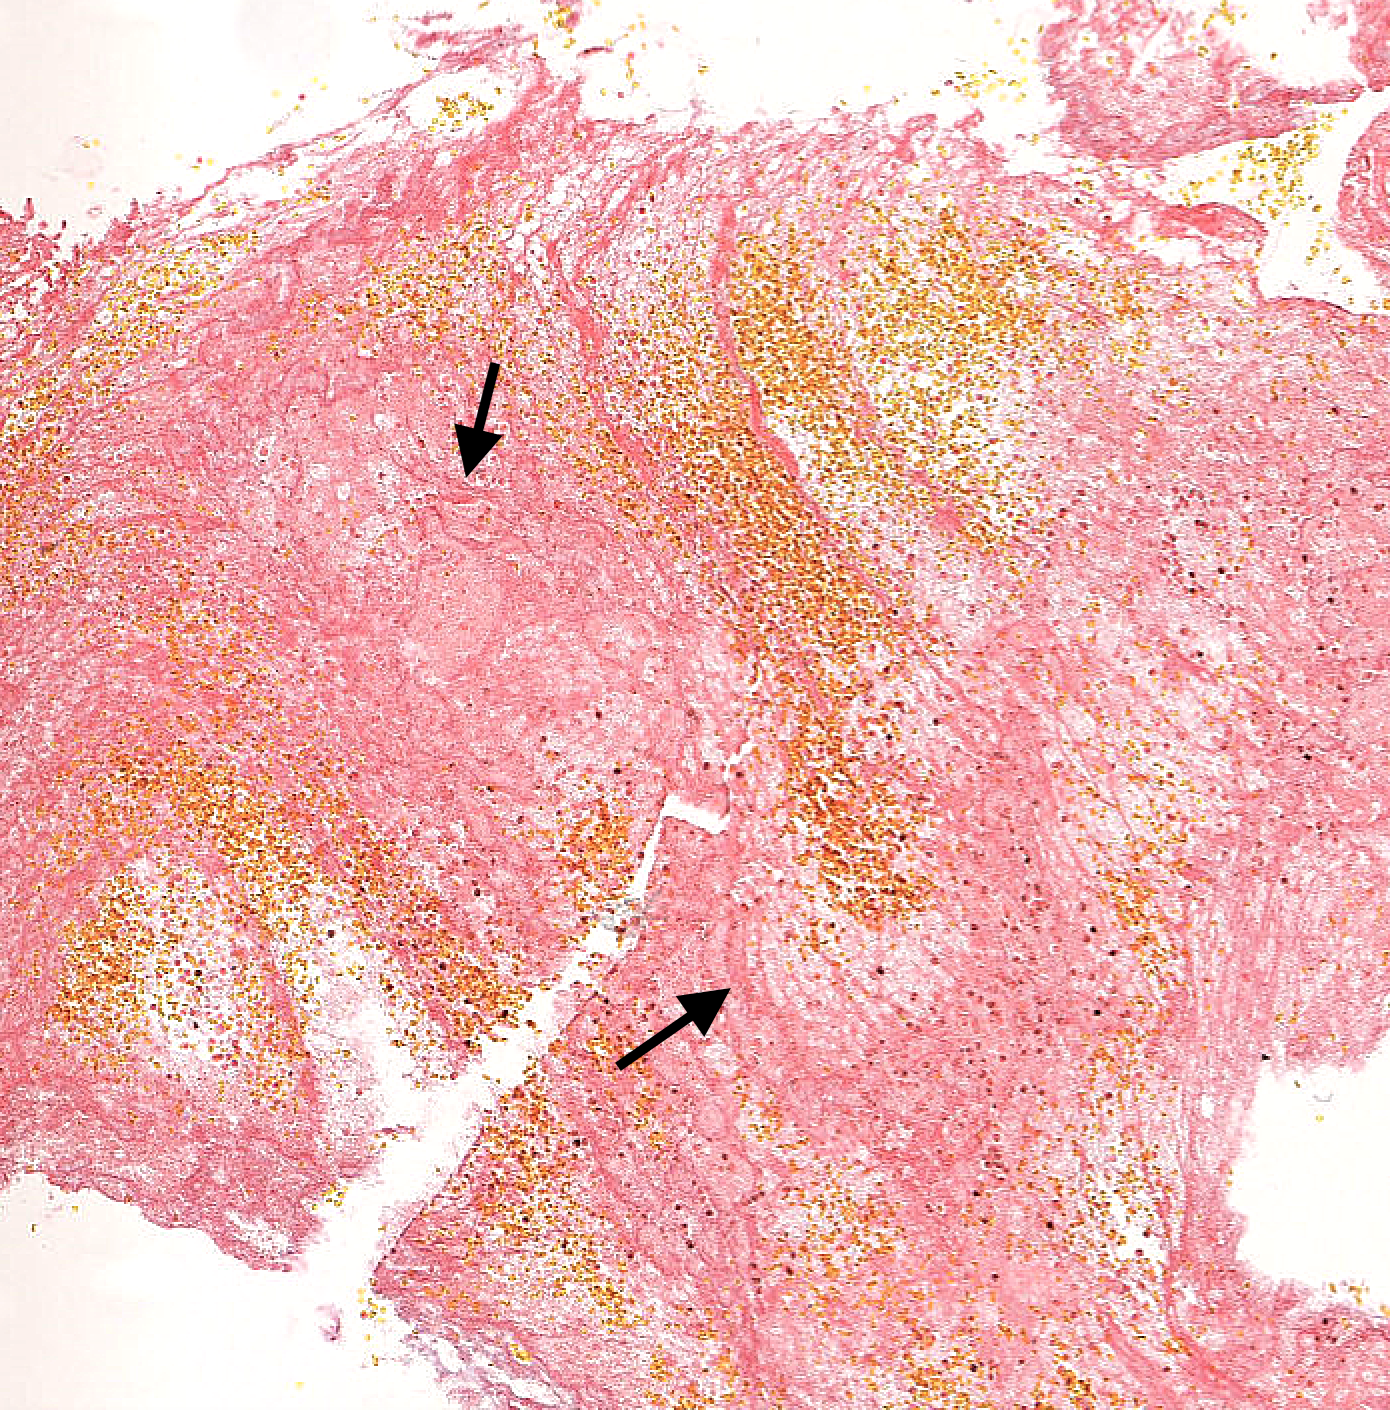
\includegraphics[width=7cm]{Indicator_vb2}}}
	
	\caption{Illustratie van de twee soorten indicator (respectievelijk paars en donkerroze) die gedetecteerd moeten worden. We zien duidelijk dat het detecteren op afbeelding (a) eenvoudiger zal zijn dan op afbeelding (b).}
	\label{figuur indicators}
\end{figure}

\section{Onze oplossing}
In dit hoofdstuk trachten we een oplossing te vinden voor ons probleem. We willen namelijk het percentage indicatorpixels in een willekeurige afbeelding kunnen berekenen. Het hoofdstuk is opgedeeld in verschillende deelproblemen: het verwijderen van de achtergrond, het lokaliseren van de indicator en de gebruiksvriendelijke app. Alle resultaten zijn bekomen met behulp van de programmeertaal MATLAB.\cite{matlab}


\subsection{Achtergrondverwijdering} \label{Achtergrondverwijdering}
Het eerste deelprobleem is het verwijderen van de achtergrond. Op de afbeeldingen is er heel wat vuiligheid te vinden. Voorbeelden hiervan zijn luchtbellen of kleine verkleuringen in de achtergrond zoals men ziet op de Figuur \ref{figuur achtergrondverwijdering}. In dit onderdeel wordt op zoek gegaan naar verschillende operaties om de grootste klonters te lokaliseren en alles wat geen klonter is uit de afbeelding te verwijderen. Dit leidt in feite tot een ruisvrije afbeelding.

\begin{figure}[H]
	\centering
	\includegraphics[width = 0.7\textwidth]{Ruis_afbeelding.png}	
	\caption{In de rechterbovenhoek zien we luchtbellen en in de onderste cirkel zien we een verkleuring. Beiden maken geen deel uit van een bloedklonter.}
	\label{figuur achtergrondverwijdering}
\end{figure}

\subsubsection{Bepalen van de beste threshold}
Om een onderscheid tussen de achtergrond en de bloedklonter te maken, wordt de afbeelding omgezet in grijswaarden(zie Figuur \ref{figuur beste_threshold}). Eén grijswaarde is nu voldoende om het onderscheid te maken. Een histogram van deze grijswaarden, zoals die weergegeven op Figuur \ref{figuur graf1}, toont aan dat er een duidelijk dipje in de frequenties tussen het wit en het grijs te zien is. Dit is dan ook de theoretisch optimale threshold, de grijswaarde om een bloedklonterpixel van een achtergrondpixel te onderscheiden. Voor deze threshold wordt het minimum van alle kleurwaarden boven de 200 genomen. Wanneer alles onder deze waarde voorgesteld wordt door een witte pixel en alles boven deze waarde door een zwarte pixel bekomt men de binaire Figuur \ref{figuur foto_bin}. De witte pixels lijken hier nagenoeg de klonters te detecteren.

\begin{figure}[H]
	\centering
	\subfloat[]{{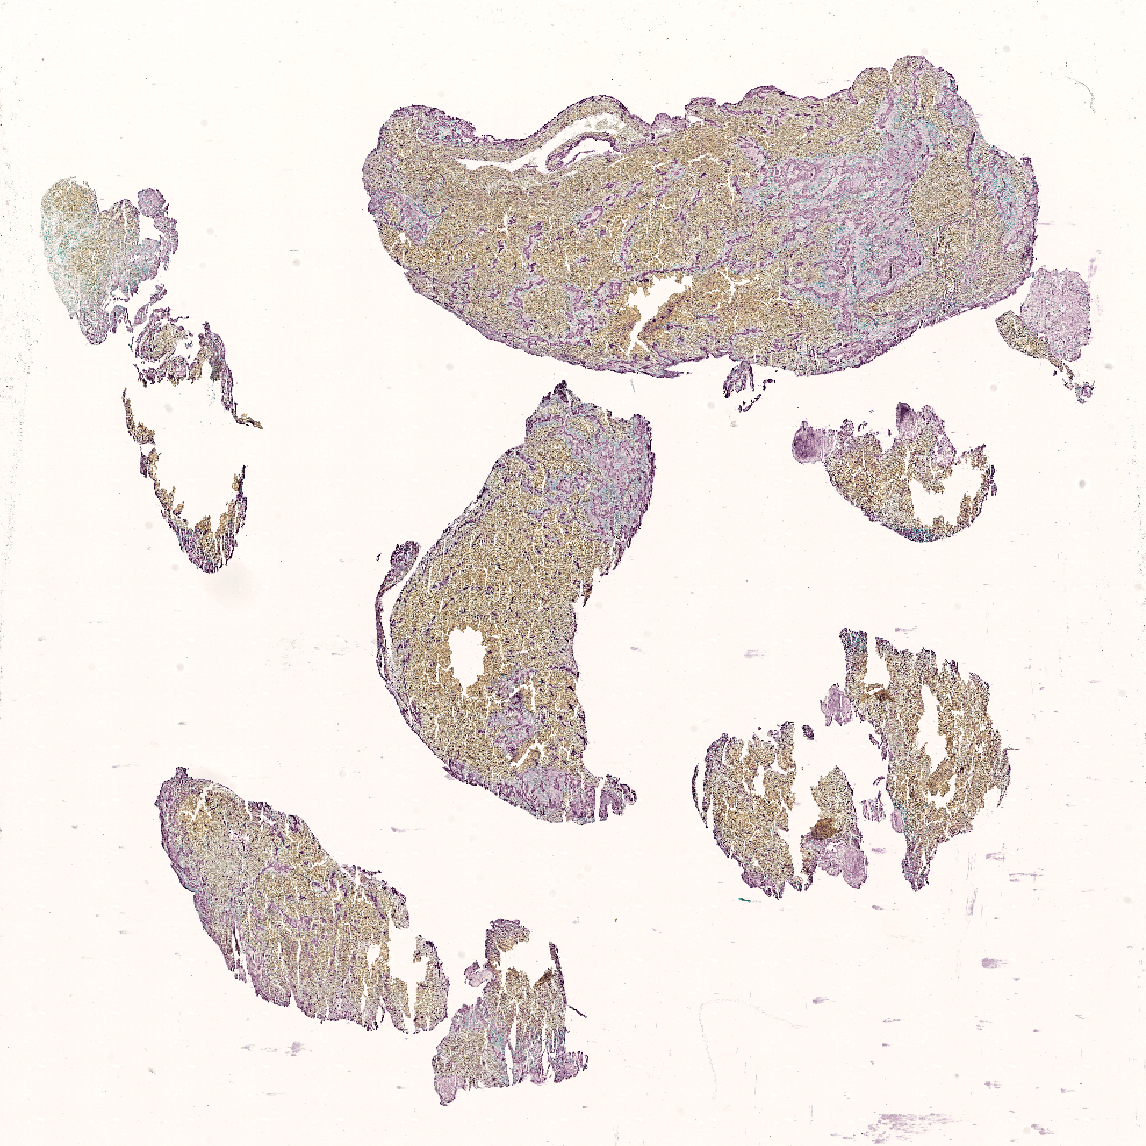
\includegraphics[width=6cm]{origineel_vb}}}
	\qquad
	\subfloat[]{{\includegraphics[width=6cm]{grijswaarden_vb}}}
	
	\caption{Illustratie van de originele foto (a) en deze omgezet in grijswaarden (b).}
	\label{figuur beste_threshold}
\end{figure}

\begin{figure}[H]
	\centering
	\includegraphics[width=0.85\textwidth]{GetBestthreshold_vb_aangeduid.png}
	
	\caption{Histogram van het aantal pixels gegroepeerd per grijswaarde. We zien duidelijk een lokaal minimum rond de waarde 230. Opmerking: we maken hier gebruik van een logaritmische y-as.}
	\label{figuur graf1}
\end{figure}

\begin{figure}[H]
	\centering
	\includegraphics[width=0.7\textwidth]{grijswaarden_bin_vb}
	\caption{Op deze binaire representatie zijn de bloedklonters duidelijk te zien.}
	\label{figuur foto_bin}
\end{figure}

\subsubsection{Ruisfilter}
Deze binaire representatie bevat echter heel wat holtes en ruis. Dit probleem kan echter simpel opgelost te worden door alle kleine groepen zwarte pixels te vervangen door witte. Deze eerste stap vult voornamelijk alle holtes in de bloedklonters op. Daarnaast worden ook alle kleine groepen witte pixels vervangen door zwarte pixels. Bijgevolg verdwijnen alle alleenstaande pixels die voornamelijk ruis zijn. Het resultaat van deze operatie is te zien op Figuur \ref{figuur ruisfilter} (a). \\
Deze binaire afbeelding noemt men een 'mask'. Die 'mask' wordt als filter bovenop de originele afbeelding gelegd. Hierbij worden alle zwarte pixels op de mask vervangen door witte pixels op de originele afbeelding en alle witte pixels op de mask behouden door hun kleur op de originele afbeelding. Daarnaast wordt de afbeelding nog bijgesneden om kostbare geheugenruimte te sparen. Het uiteindelijke resultaat is te zien op de afbeelding in Figuur \ref{figuur ruisfilter} (b). In dit deelprobleem werd echter met een reeds bijgesneden bloedklonter gewerkt om de afbeeldingen duidelijk te houden. Een volledig onbewerkte afbeelding is echter te zien in Figuur \ref{figuur volledig_onbewerkt}

\begin{figure}[H]
	\centering
	\subfloat[]{{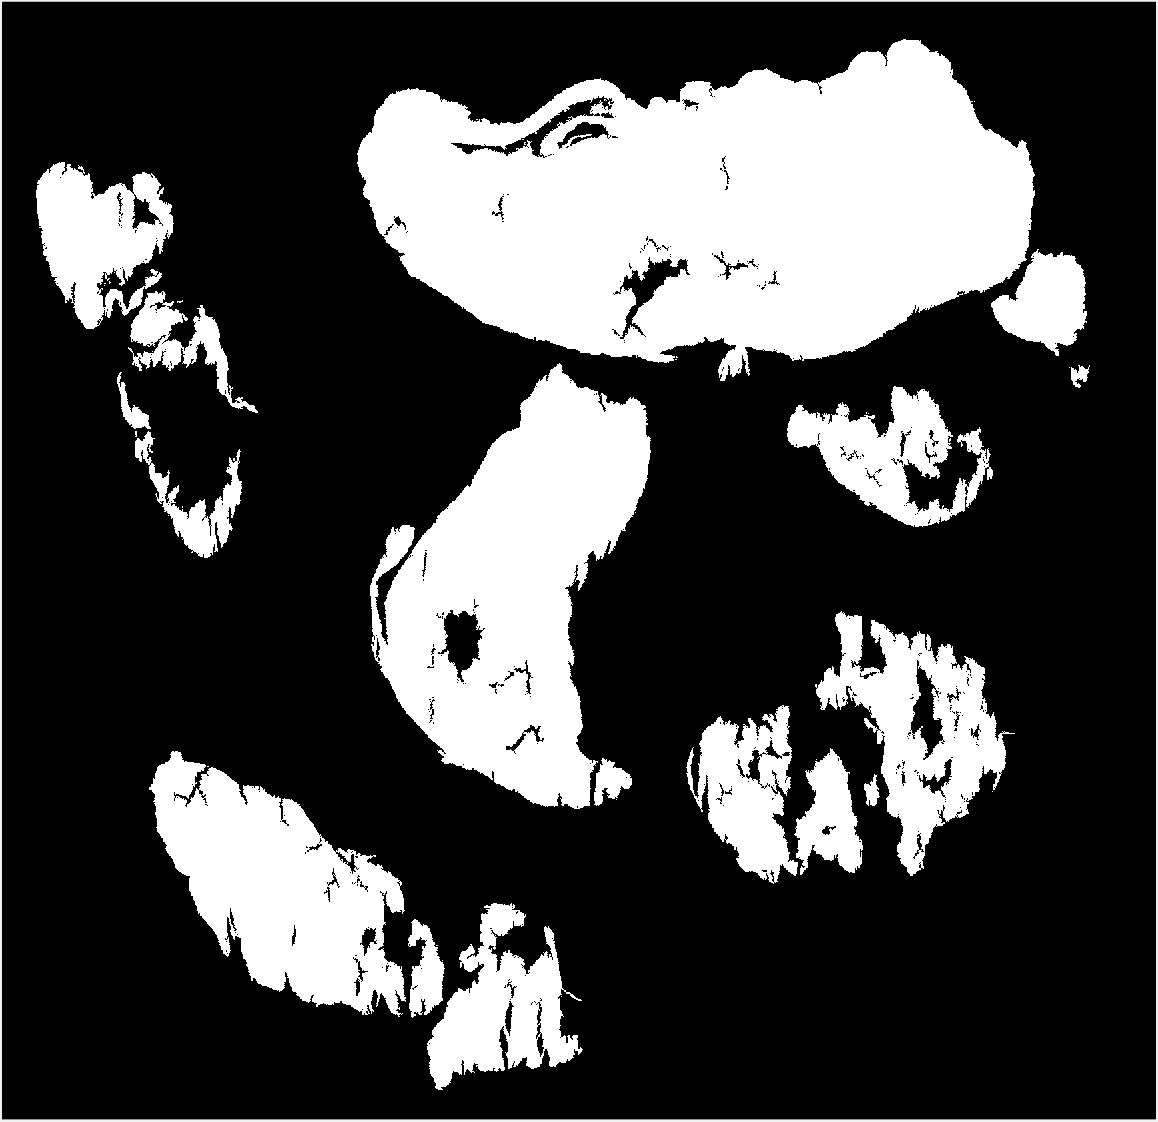
\includegraphics[width=7cm]{ruisvrij_vb}}}
	\qquad
	\subfloat[]{{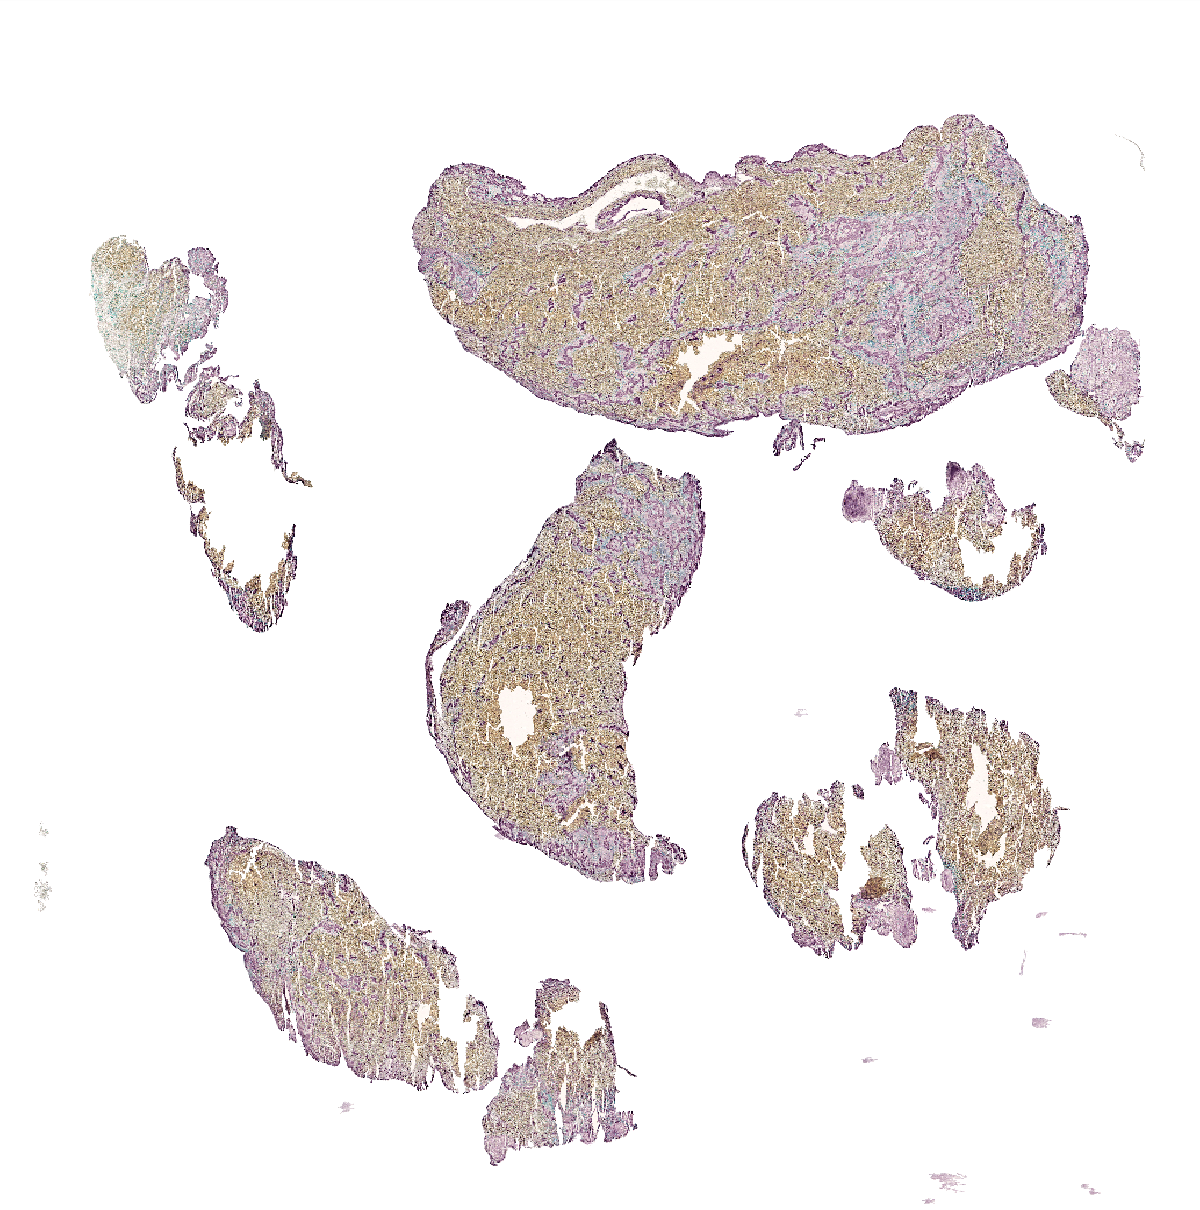
\includegraphics[width=7cm]{ruisvrij_kleur_vb}}}
	
	\caption{Alle ruis is verwijderd, dit is een foto die verder verwerkt kan worden.}
	\label{figuur ruisfilter}
\end{figure}

\begin{figure}[H]
	\centering
	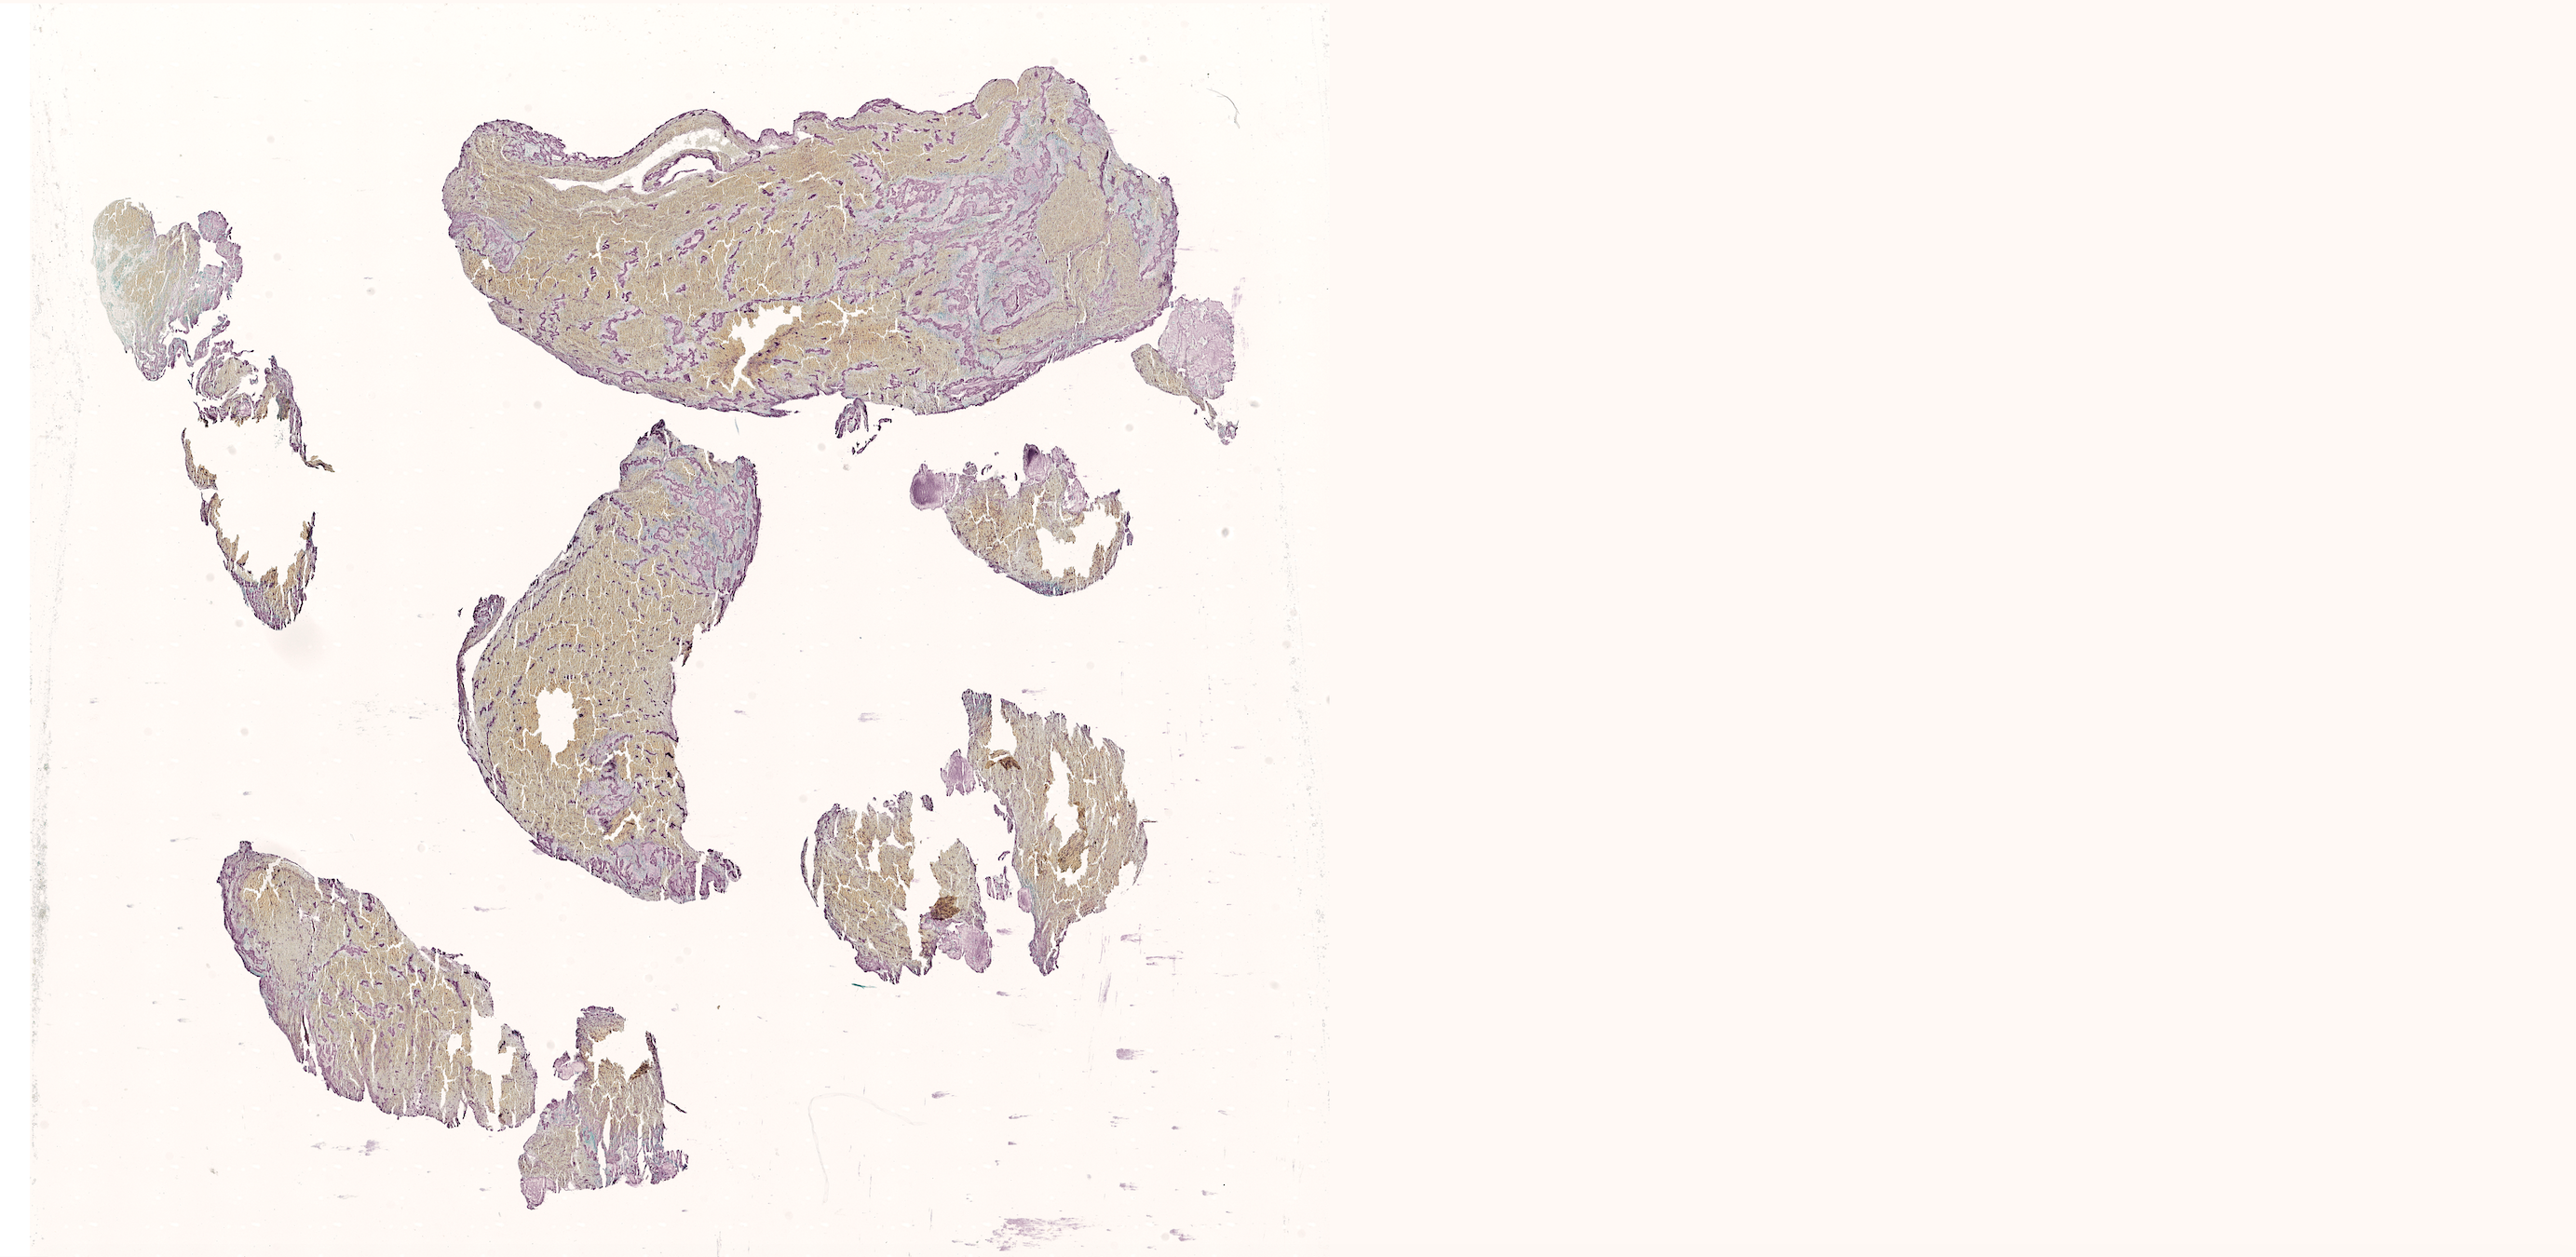
\includegraphics[width=15.25cm]{Volledig_onbewerkt}
	
	\caption{Dit is een volledig onbewerkte afbeelding die we in \ref{figuur ruisfilter} (b) hebben bijgesneden en waarvan de achtergrond verwijderd is.}
	\label{figuur volledig_onbewerkt}
\end{figure}

\subsubsection{Uitzonderingen}
Naast de gewone bloedklonters zijn er ook nog enkele uitzonderingen. Sommige klonters hebben namelijk geen rode bloedcellen waardoor ze zeer wit zijn, zoals te zien is op Figuur \ref{figuur lichte_kleuring}. Het probleem is dat hier geen optimale threshold te berekenen valt. Er is namelijk een zeer kleine afstand tussen de kleur van de bloedklonter en de feitelijke achtergrond. Vandaar dat in de app een slider verwerkt is om desnoods zelf die threshold aan te aanduiden. Wanneer de optimalisaties van de simpele binaire mask daarna op deze threshold toegepast worden, bekomt men Figuur \ref{figuur lichte_kleuring_binair}. Het is duidelijk te zien dat dit algoritme zeer krachtig is wanneer een goede threshold gekend is.

\begin{figure}[H]
	\centering
	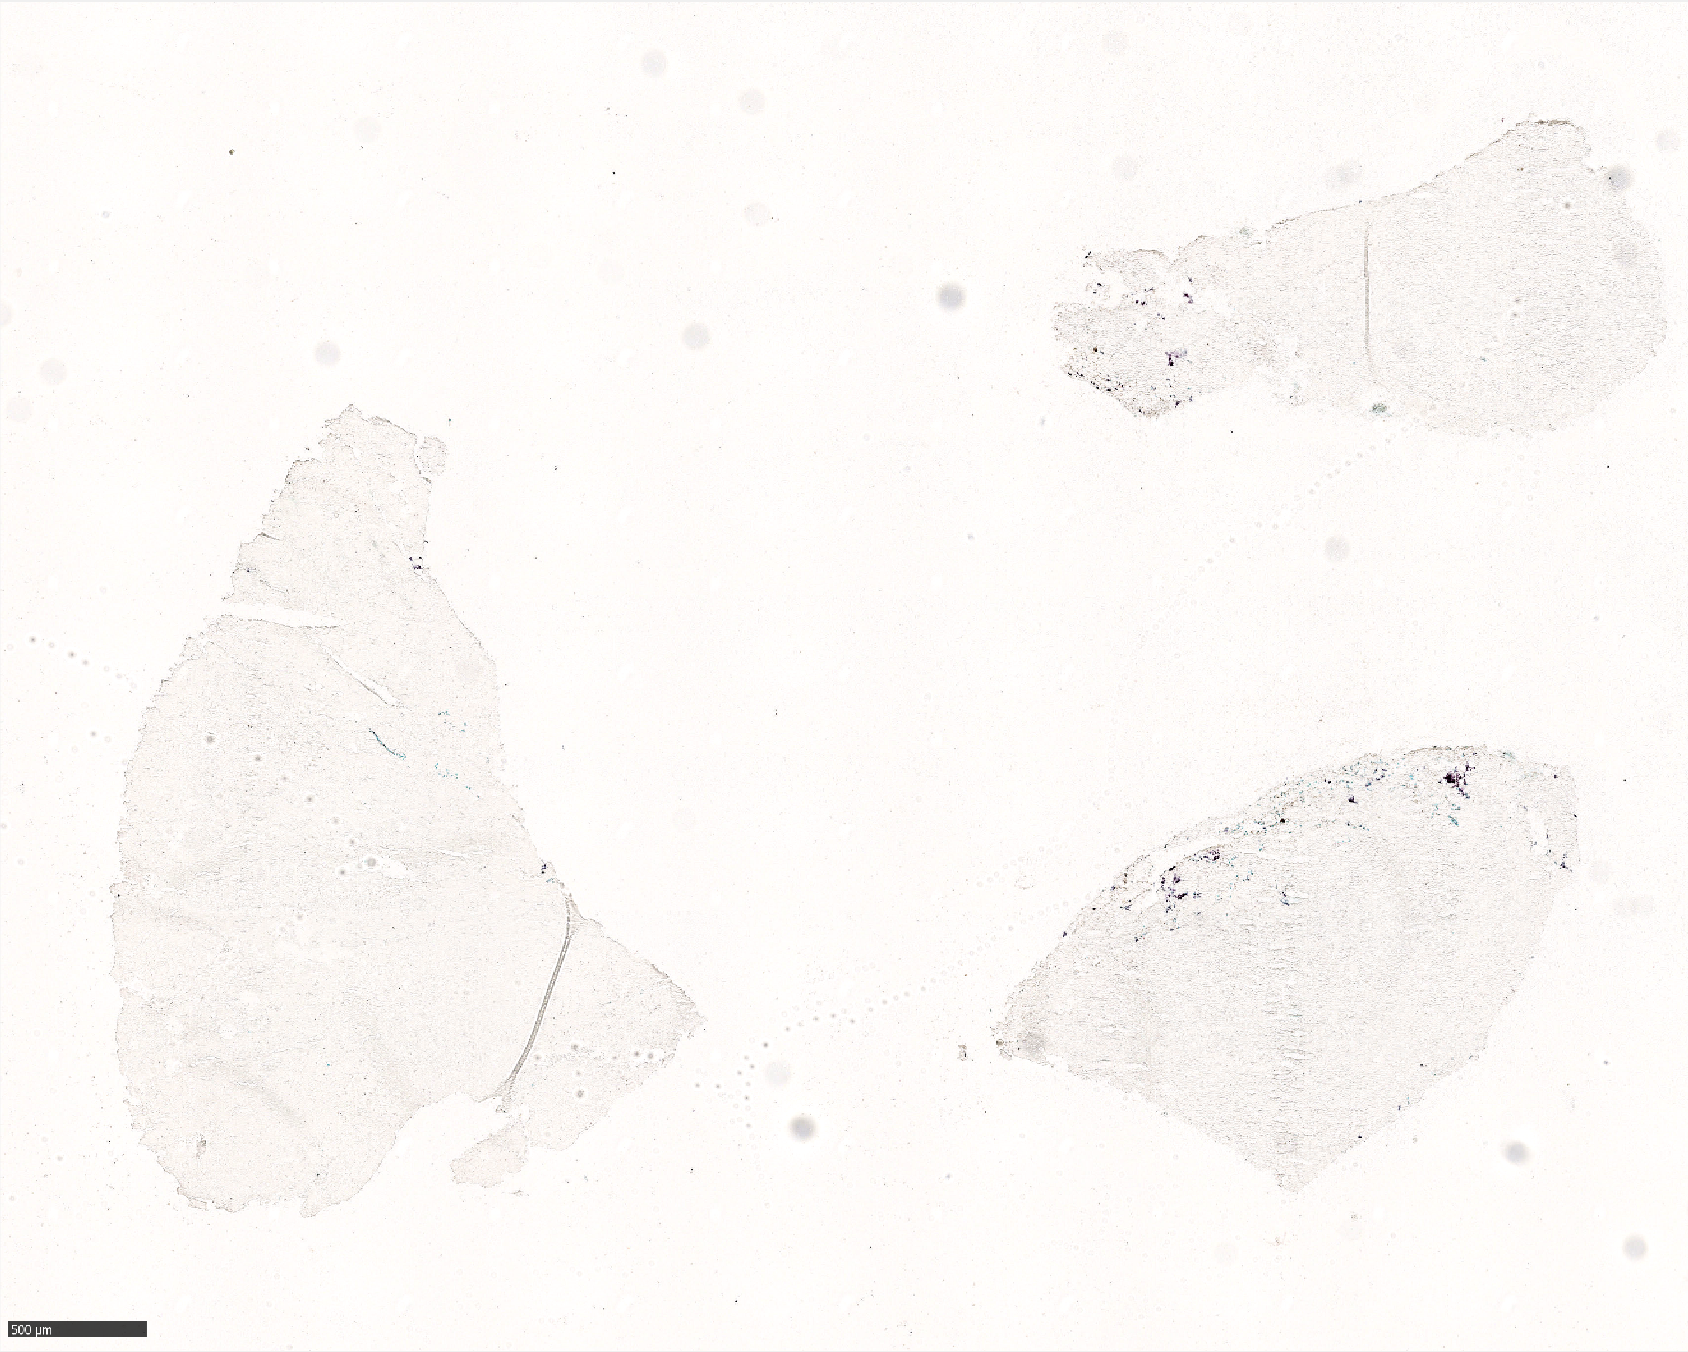
\includegraphics[width=0.7\textwidth]{lichte_kleuring}
	
	\caption{Een afbeelding van een bloedklonter zonder rode bloedcellen.}
	\label{figuur lichte_kleuring}
\end{figure}

\begin{figure}[H]
	\centering
	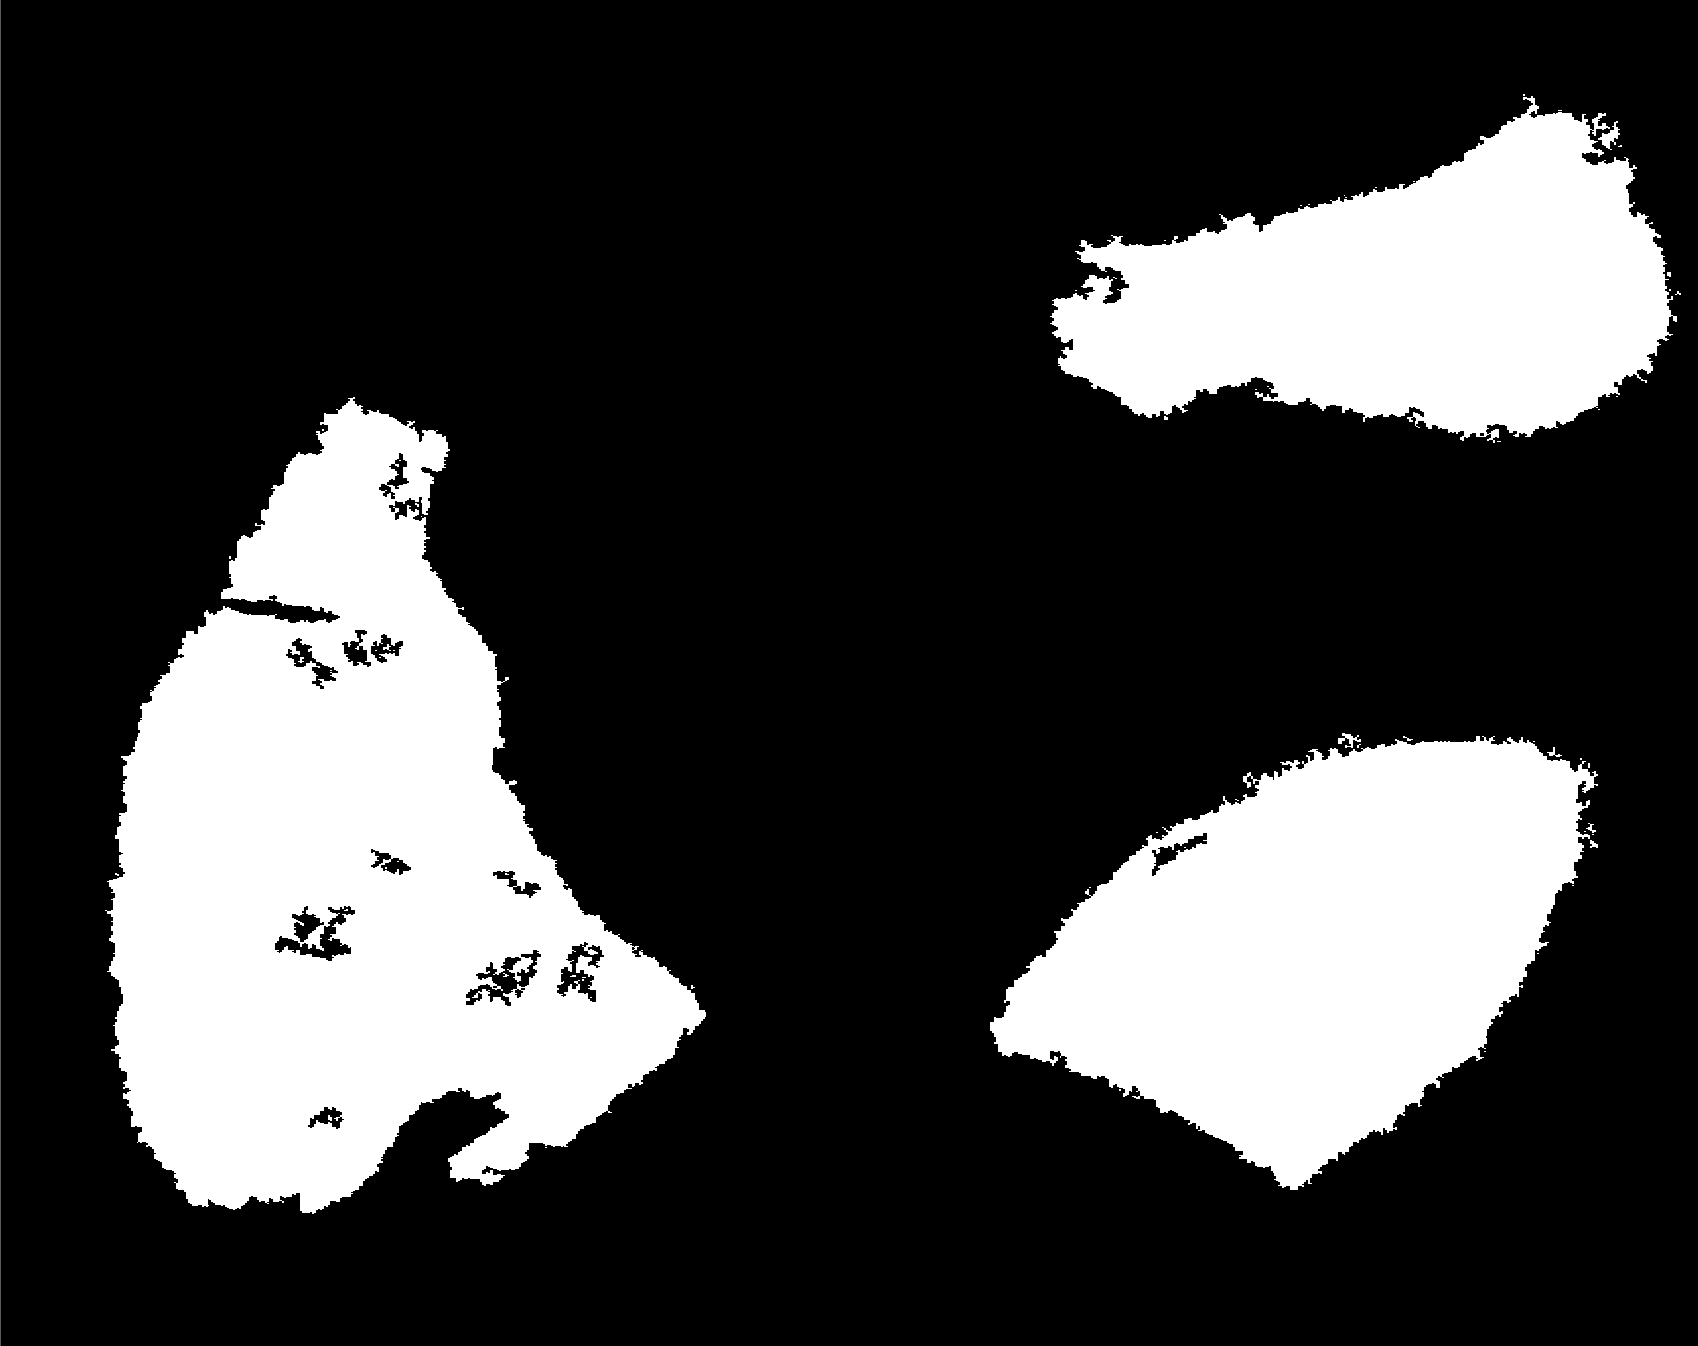
\includegraphics[width=0.7\textwidth]{lichte_kleuring_binair}
	
	\caption{Dit is de binaire mask die we bekomen na het toepassen van de threshold en de optimalisatie van deze. De klonters worden nu met zekere precisie aangeduid.}
	\label{figuur lichte_kleuring_binair}
\end{figure}


\subsection{Lokalisatie van de indicator} \label{lokalisatie_indicator}
Het tweede deel van het project is de indicators lokaliseren en kwantificeren. Hierbij moet de code in staat zijn twee specifieke soorten van indicatoren te onderscheiden. Van deze is een voorbeeld op Figuur \ref{figuur indicators} te zien. Omdat het kleurverschil tussen wat aangeduid moet worden (indicator) en wat niet (achtergrond) niet altijd even groot is, wordt het oorspronkelijke \textit{RGB} kleurmodel\footnote{Het RGB kleurmodel is een voorstelling waarbij ieder kleur voorgesteld wordt door een waarde van de drie basiskleuren (rood, groen en blauw)} omgevormd naar het zogenaamde \textit{HSV} kleurmodel. Dit model is een alternatieve voorstelling waarbij men alle kleuren op een cirkel zoals in Figuur \ref{figuur hsv_schema} voorstelt, de hoek die dit kleur dan maakt, noemt men de \textit{Hue}. Naast deze waarde heeft \textit{HSV} nog twee andere parameters namelijk \textit{Saturation} en \textit{Value}. \textit{Saturation} kan simpel beschouwd worden als een aanduiding van de hoeveelheid witte kleur en \textit{Value} een aanduiding van de zwarte kleur.\\
Het voordeel van deze transformatie is dat het heel wat eenvoudiger is om een onderscheid tussen dichtbijgelegen kleuren te vinden. Andere mogelijke transformaties zijn die naar het \textit{LAB} of het \textit{CMYK} kleurmodel die gelijkaardige eigenschappen hebben en desnoods ook gebruikt kunnen worden. Eenmaal een duidelijk onderscheid tussen de indicator en de achtergrond gemaakt is, wordt het percentage indicator eenvoudig berekend als de verhouding van het aantal bloedklonter- en indicatorpixels. Ons stappenplan wordt in dit hoofdstuk besproken en toegepast op de afbeelding uit Figuur \ref{figuur indicators} (a). Maar kan evenwel gebruikt worden op een andere kleuring met weliswaar andere beginwaarden.

\begin{figure}[H]
	\centering
	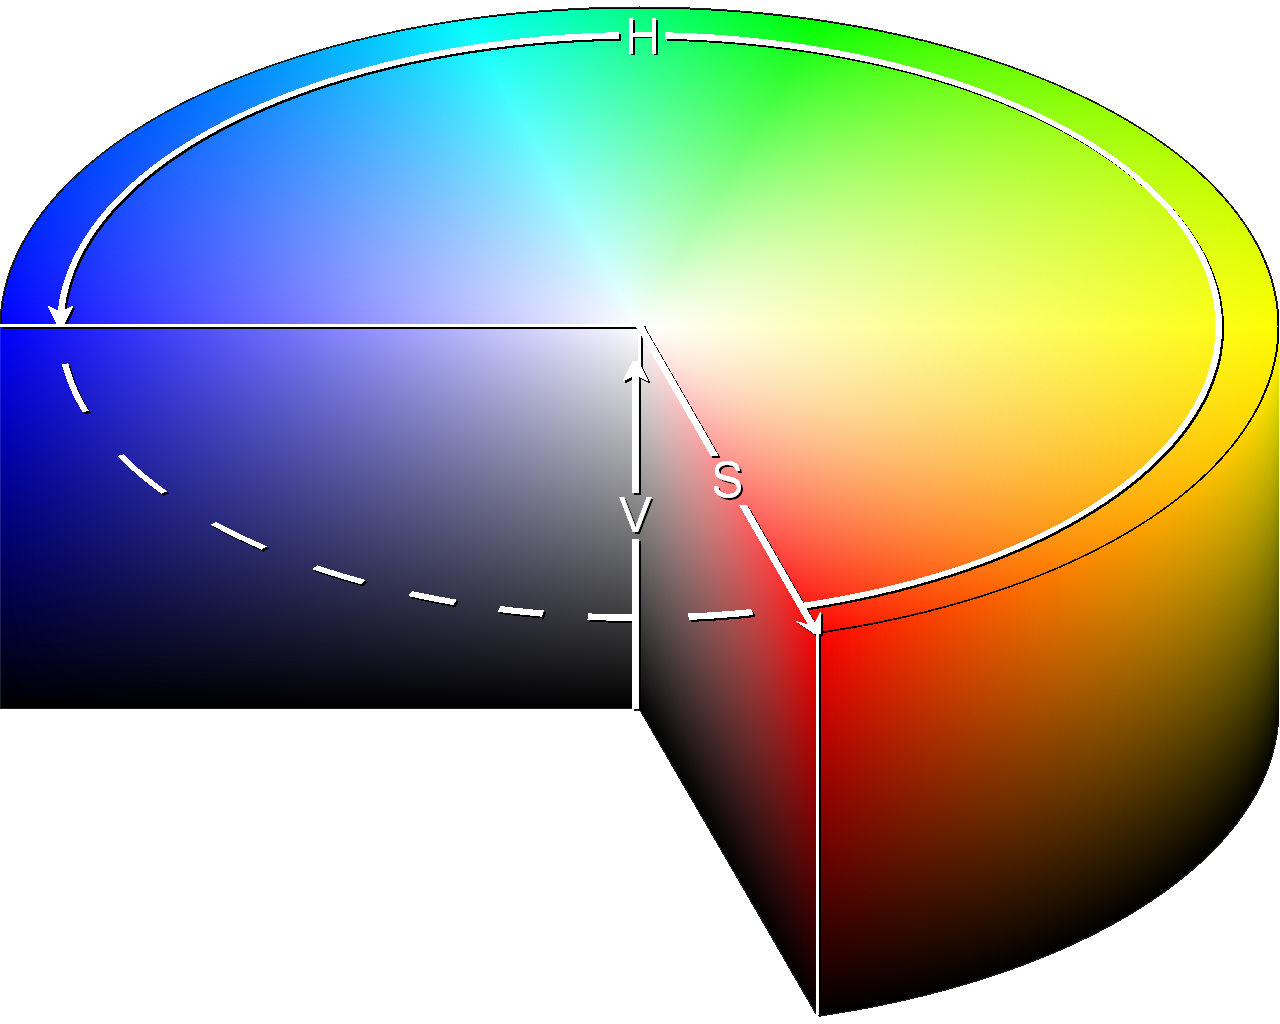
\includegraphics[width=0.7\textwidth]{HSV_vb.png}
	
	\caption{Grafische voorstelling van het \textit{HSV} (\textit{Hue}, \textit{Saturation}, \textit{Value}) kleurmodel\cite{hsvcolspace}}
	\label{figuur hsv_schema}
\end{figure}

\subsubsection{Het HSV kleurmodel}
Zoals reeds vermeld, wordt eerst een transformatie naar het \textit{HSV} kleurmodel uitgevoerd. Een vergelijking tussen de twee voorstellingen is te zien in de Figuren \ref{figuur RGB} en \ref{figuur HSV}. Het model is telkens ontbonden in de drie kleurwaarden, waarbij zwart de laagste waarde voor dat kleur voorstelt en wit de hoogste. Het verschil tussen de twee kleurmodellen is duidelijk te zien. Afbeelding (a) en (b) uit Figuur \ref{figuur HSV} lijken namelijk een iets agressiever onderscheid te maken tussen de verschillende kleuren in de originele afbeelding.

\begin{figure}[H]
	\centering
	\subfloat[]{{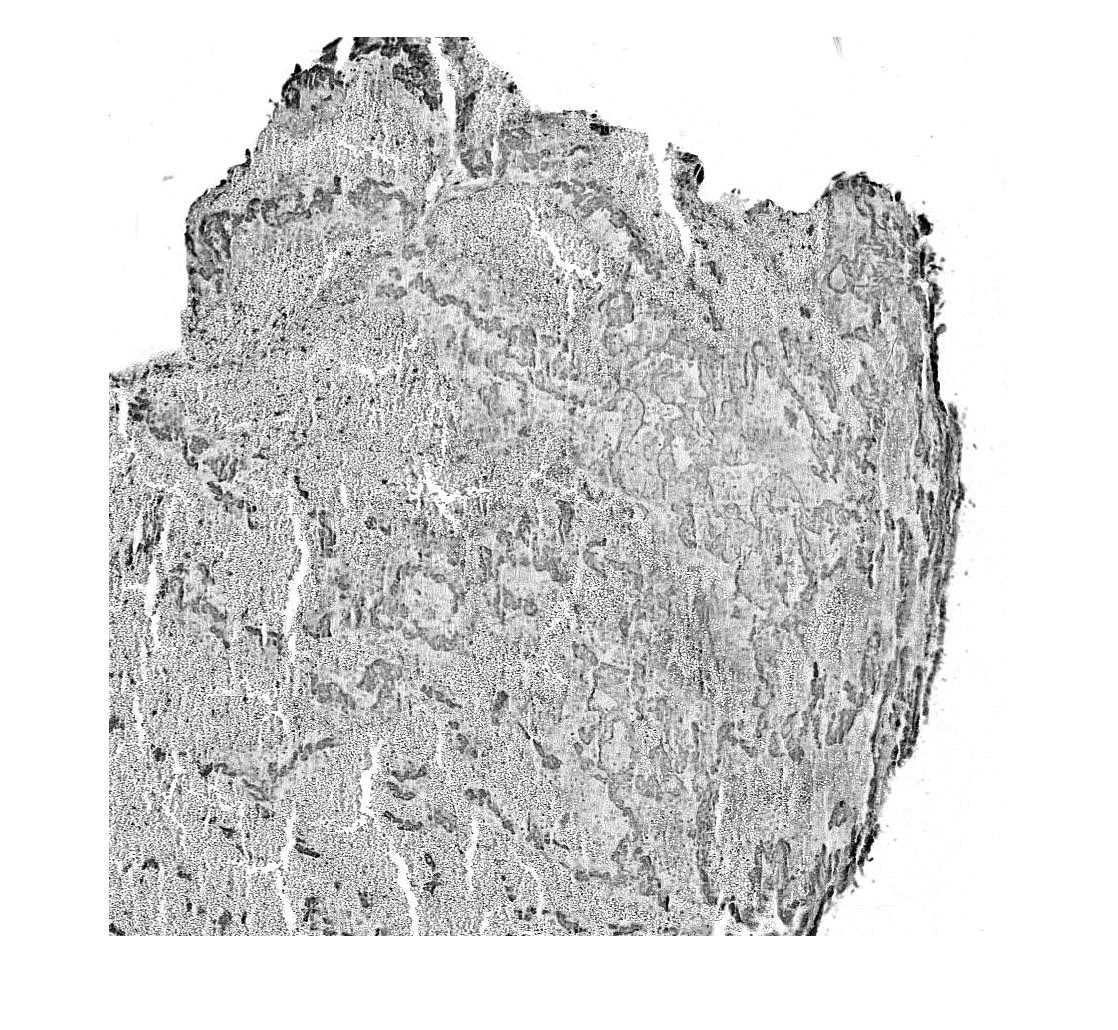
\includegraphics[width=4.5cm]{RGB_r}}}
	\qquad
	\subfloat[]{{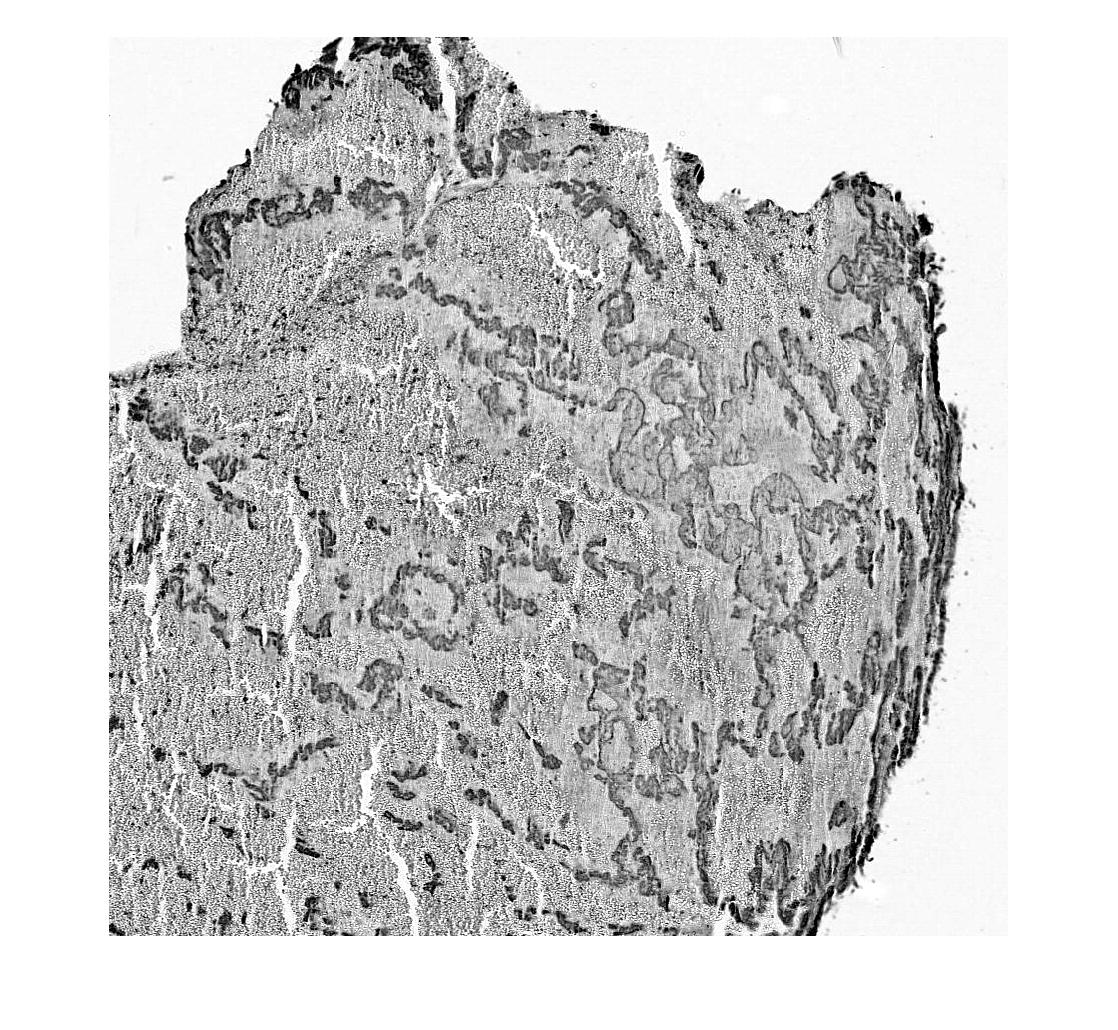
\includegraphics[width=4.5cm]{RGB_g}}}
	\qquad
	\subfloat[]{{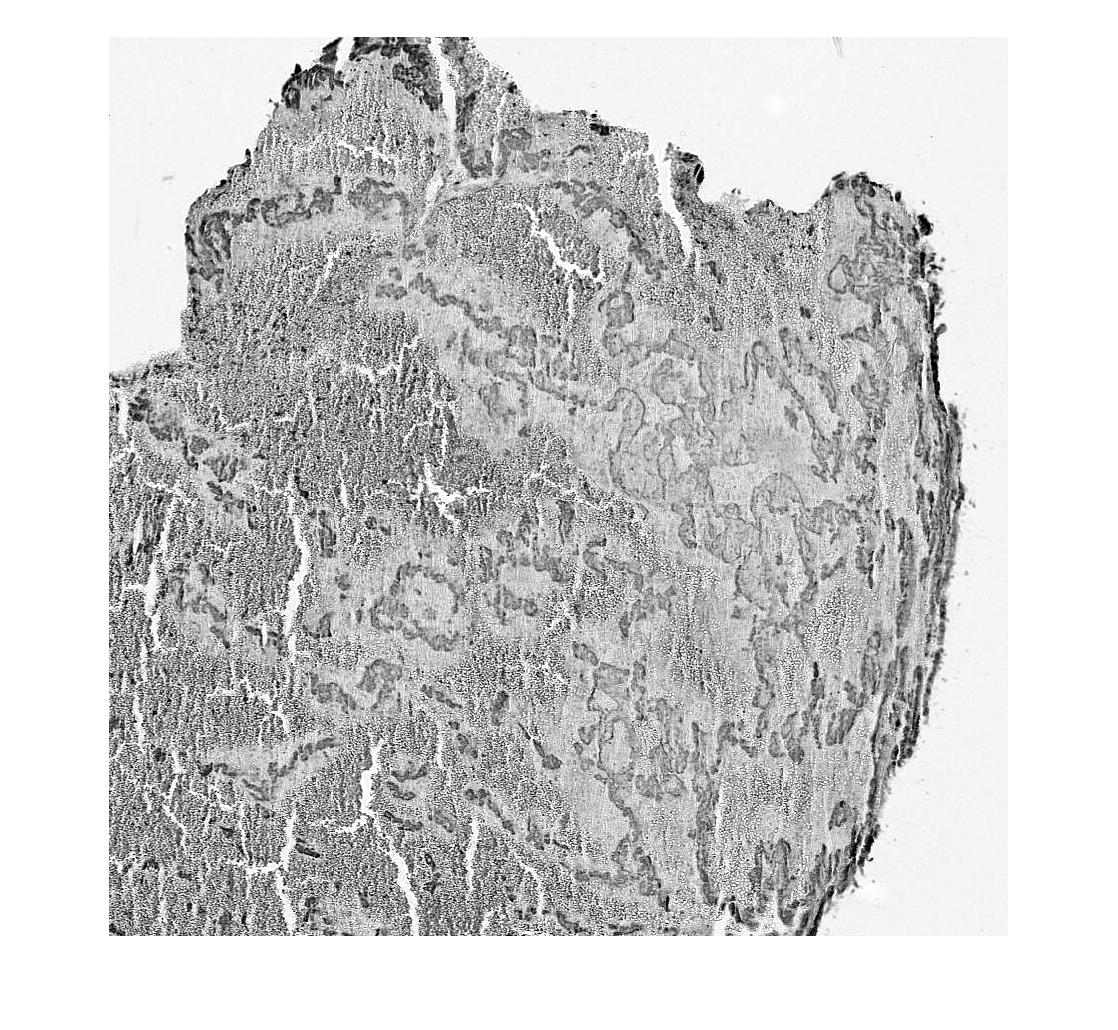
\includegraphics[width=4.5cm]{RGB_b}}}
	\caption{Illustratie van respectievelijk de rode, groene en blauwe kleurwaarden (\textit{RGB}). Hierbij komt wit overeen met de maximumwaarde en zwart met de minimumwaarde van die kleur.}
	\label{figuur RGB}
\end{figure}

\begin{figure}[H]
	\centering
	\subfloat[]{{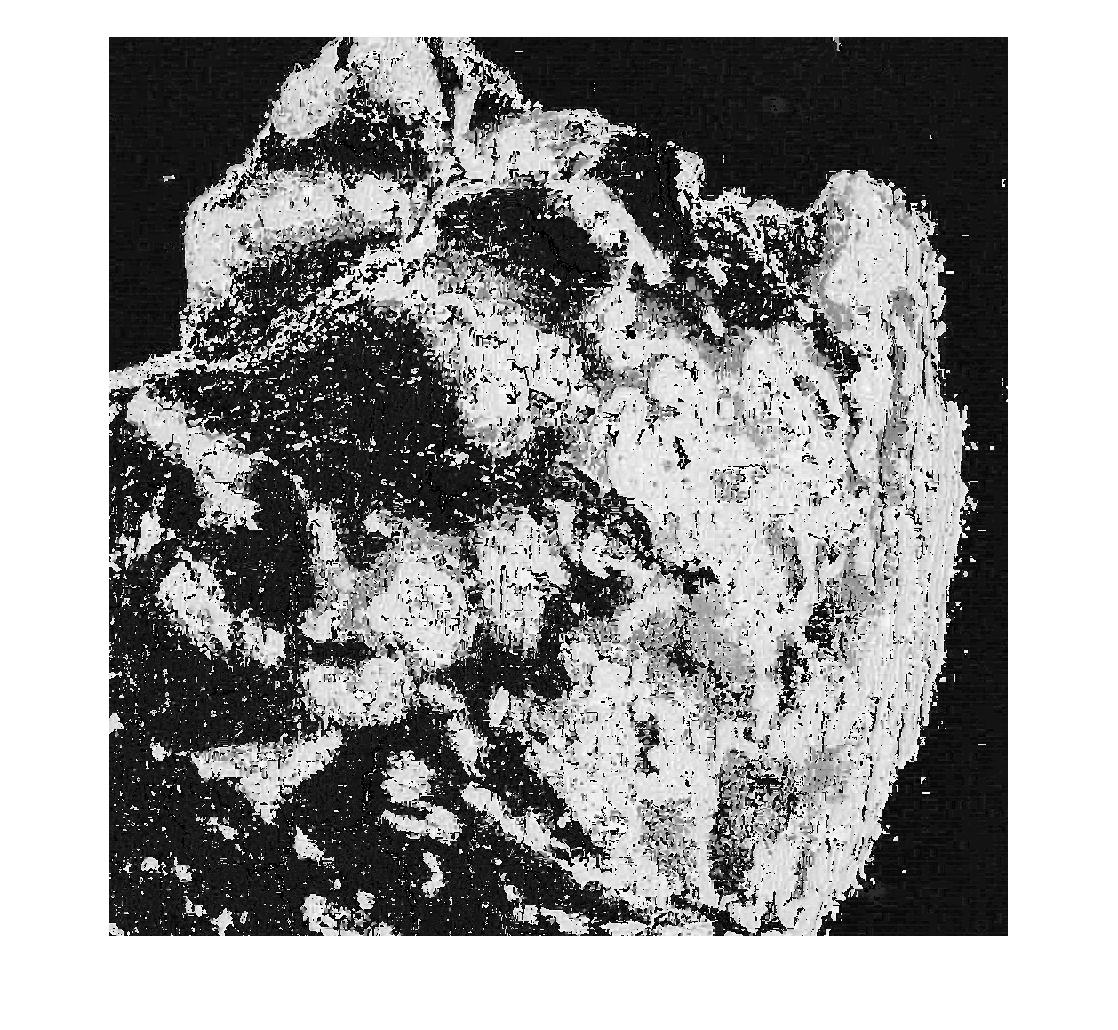
\includegraphics[width=4.5cm]{HSV_h}}}
	\qquad
	\subfloat[]{{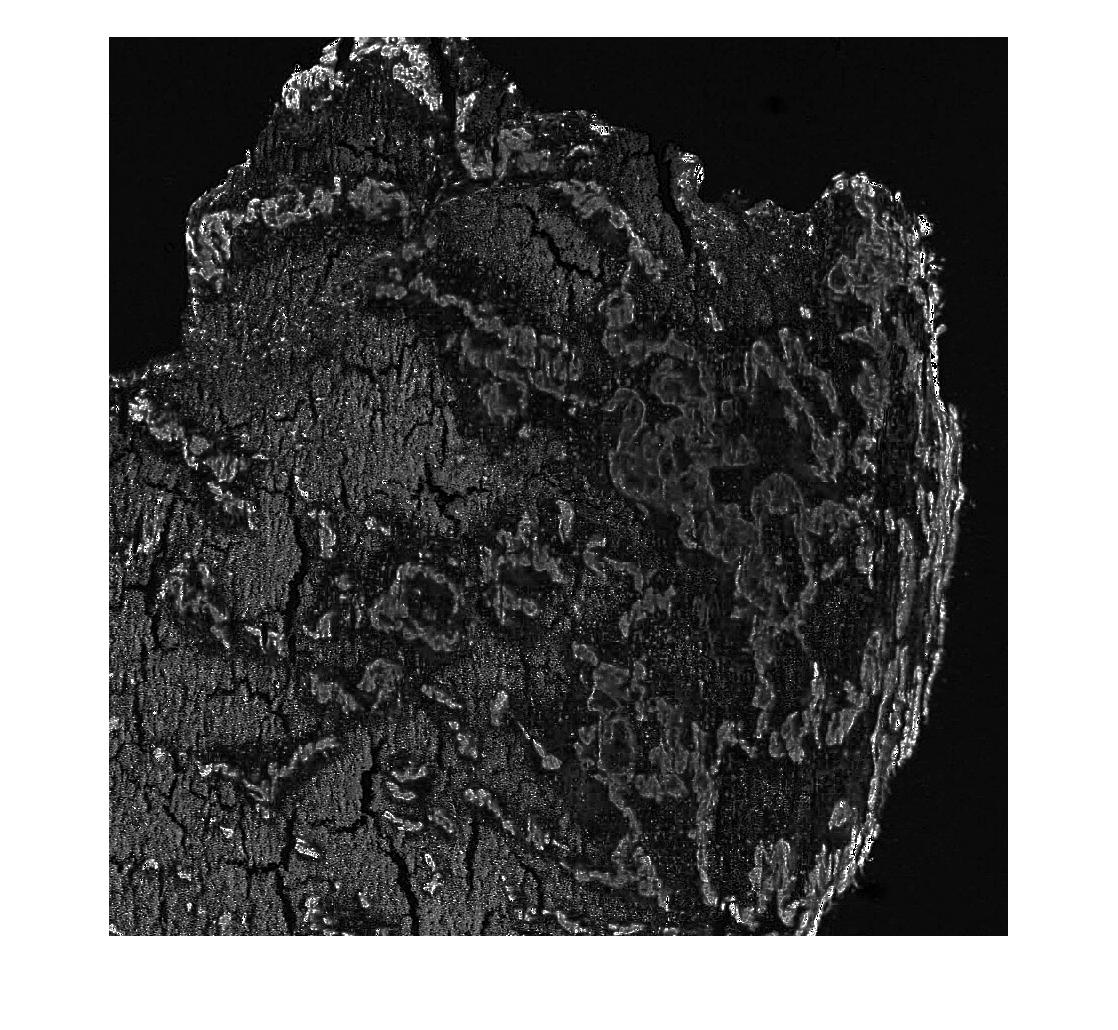
\includegraphics[width=4.5cm]{HSV_s}}}
	\qquad
	\subfloat[]{{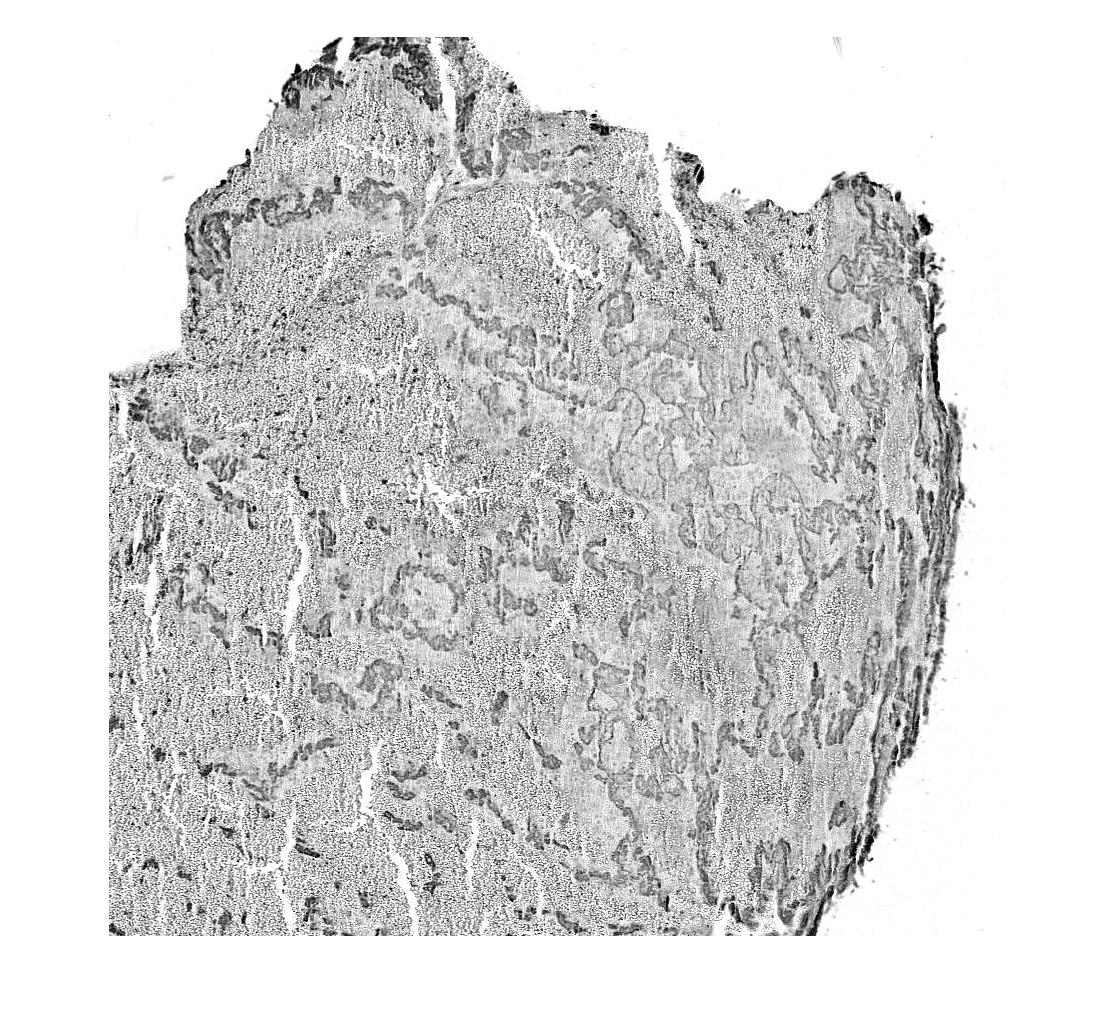
\includegraphics[width=4.5cm]{HSV_v}}}
	
	\caption{Illustratie van respectievelijk de \textit{hue}, \textit{saturation} en \textit{value} kleurwaarden (\textit{HSV}). Hierbij komt wit overeen met de maximumwaarde en zwart met de minimumwaarde van die kleurwaarde.}
	\label{figuur HSV}
\end{figure}

\subsubsection{Een algemene threshold}
De volgende stap is een filter bepalen voor de indicatorpixels. Het probleem is echter dat een goede filter voor de ene afbeelding niet altijd een goede filter voor de andere is. Daarom werd voor iedere afbeelding afzonderlijk manueel een minimum- en maximumwaarde voor elke kleurwaarde bepaald. Daarna werd het minimum van deze minimumwaarden en het maximum van deze maximumwaarden berekend. Het resultaat is een vrij algemene threshold die alle indicatorpixels met zekerheid aanduidt. Een voorbeeld is te zien op Figuur \ref{figuur alg_tresh}. Het enigste probleem is dat bepaalde pixels nu wel verkeerd aangeduid worden. Het aantal is weliswaar niet zo groot, maar aangezien ze in elke afbeelding voorkomen zullen we dit trachten te omzeilen.
\begin{figure}[H]
	\centering
	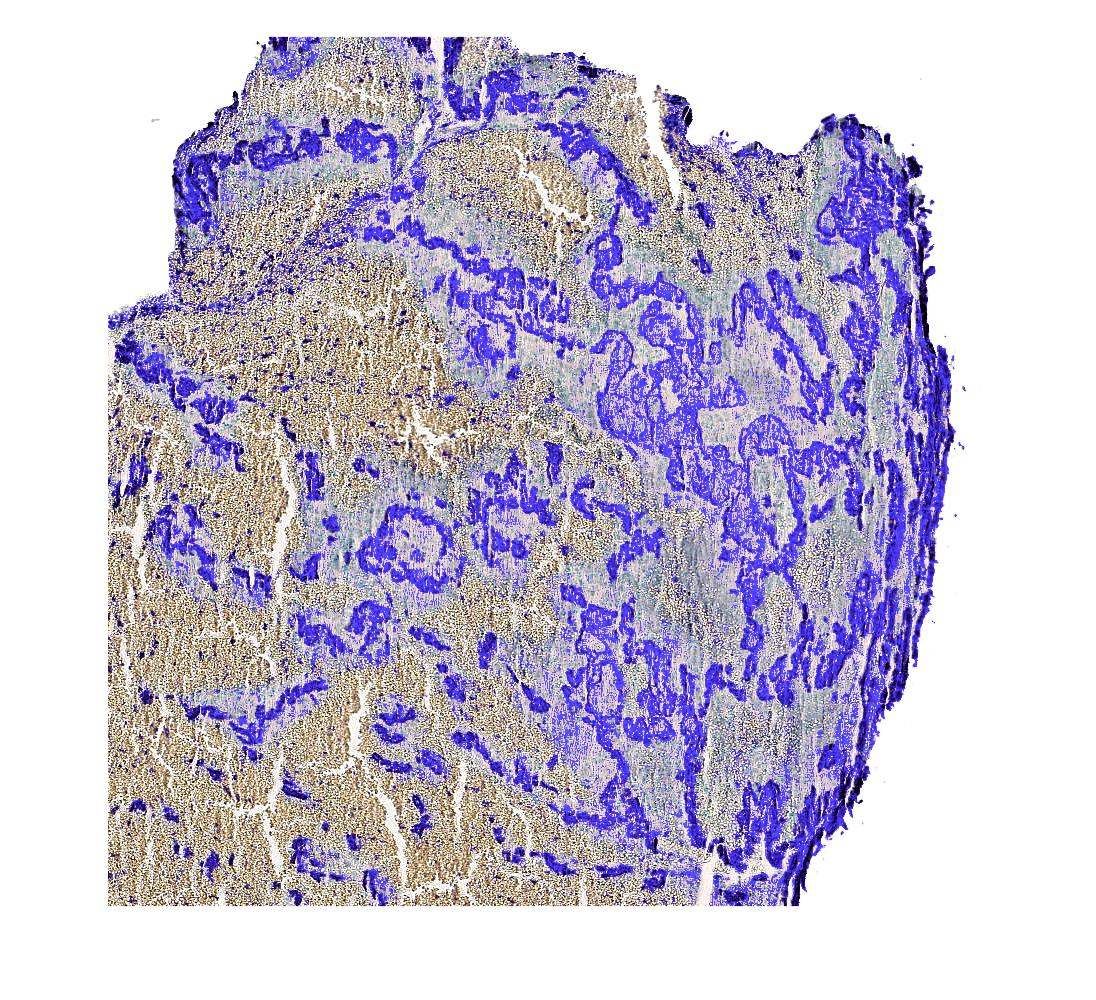
\includegraphics[width = 0.7\textwidth]{algemene_threshold}
	
	\caption{We hebben alle indicatoren met een blauwe kleur aangeduid. De algemene threshold selecteert alle indicatorpixels, maar jammer genoeg ook enkele verkeerde, deze zijn aangeduid met een pijl.}
	\label{figuur alg_tresh}
\end{figure}

\subsubsection{Optimalisatie van de threshold} \label{additional_filter}
In dit hoofdstuk wordt een poging gedaan om het aantal verkeerde pixels te verminderen zonder de juiste te beïnvloeden. Aangezien reeds een vrij correcte threshold bepaald is, kan een statistische analyse van wat onder de bijhorende mask ligt, uitgevoerd worden. Wanneer een histogram van deze \textit{HSV} kleurwaarden (zie Figuur \ref{figuur HSVHIST}) opgesteld wordt, zijn duidelijke verschillen in de frequenties van een bepaalde kleurwaarde zichtbaar.\\
Het idee is om nu de verkeerde pixels via deze diagrammen eruit te filteren. Hiervoor wordt verondersteld dat deze pixels essentieel in kleur verschillen van indicatorpixels. Daarnaast komen de verkeerde pixels minder vaak voor dan de indicatorpixels. De frequentie van hun kleurwaarde is dus lager. De huidige threshold zou dus in feite manueel bijgestuurd kunnen worden. Dit heeft echter geen zin aangezien de grafieken van verschillende afbeeldingen niet volledig gelijk zijn. Ze hebben namelijk eenzelfde vorm, maar hun pieken liggen soms meer dan 5\% verschoven. Daarom passen we op iedere afbeelding afzonderlijk automatisch een filter toe. In principe kunnen alle pixels met een frequentie onder een bepaalde grenswaarde geschrapt worden. Maar een betere benadering is om het punt te vinden, waar de frequentie van de pixels enorm begint toe te nemen. Indien we deze thresholdwaarde naar de pieken toeschuiven, zijn we eigenlijk grote 'indicatoraders' aan het verwijderen. Dit zien we op Figuur \ref{figuur HSVHIST_aangeduid}. Dit punt kan theoretisch benaderd worden als het maximum van de tweede afgeleide naar de kleurwaarde. \\
Wanneer we deze filter toepassen, krijgt men het resultaat dat te zien is op Figuur \ref{figuur morf} (a). De zones die eerder verkeerd werden aangeduid zijn nu bijna volledig verdwenen.\\
Een extra stap die ten slotte toegepast wordt, is het morfologisch sluiten van de pixels. Dit door indicatorpixels die niet ver van elkaar gelegen zijn met elkaar te verbinden. Het is namelijk zo dat wanneer een pixel omringt is door indicatorpixels, de kans hoog is dat deze pixel ook een indicatorpixel is. Het resultaat is te zien op \ref{figuur morf} (b).\\
De laatste stap die nu nog rest is het optellen van alle aangeduide pixels en de bloedklonterpixels. De verhouding hiervan is bijgevolg het percentage indicator, wat net gevraagd werd.


\begin{figure}[H]
	\centering
	\subfloat[]{{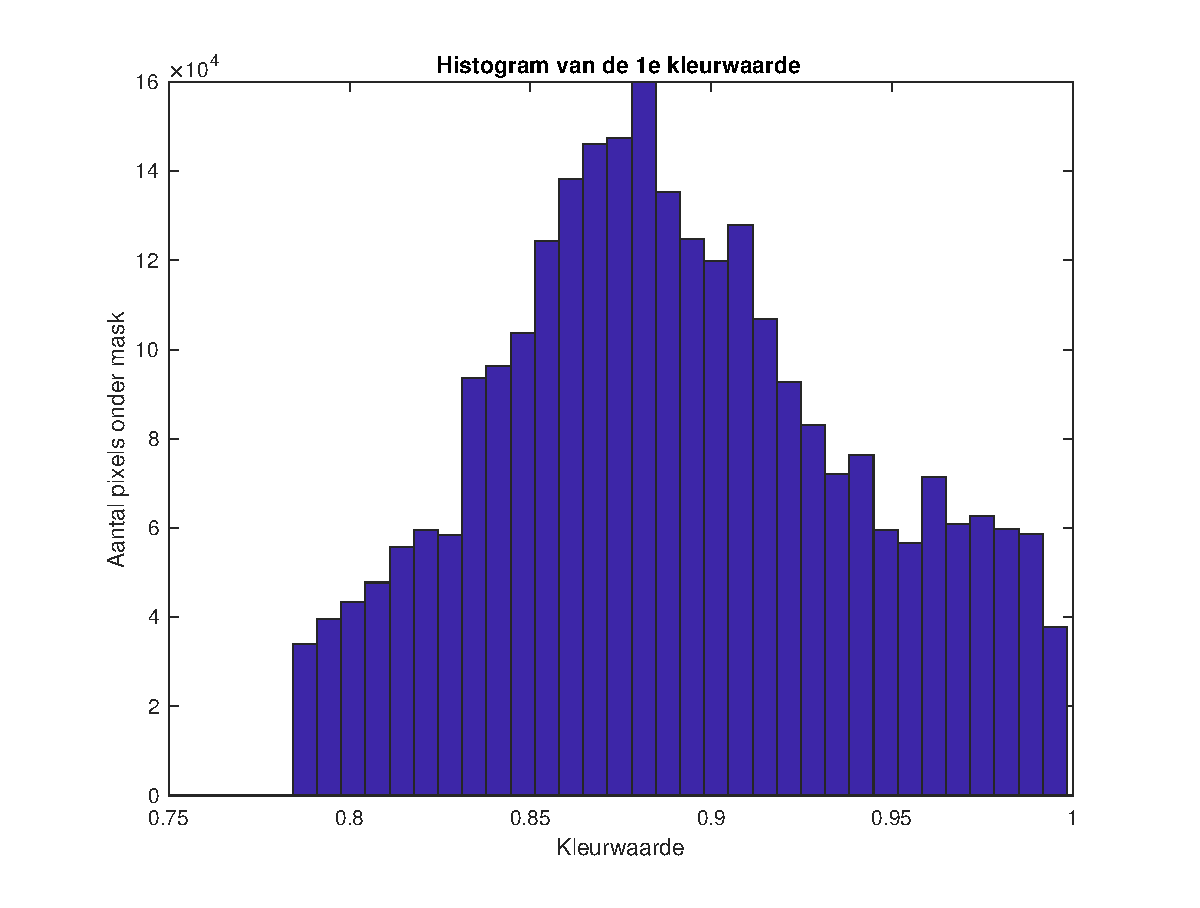
\includegraphics[width=4.5cm]{hsvhist_h}}}
	\qquad
	\subfloat[]{{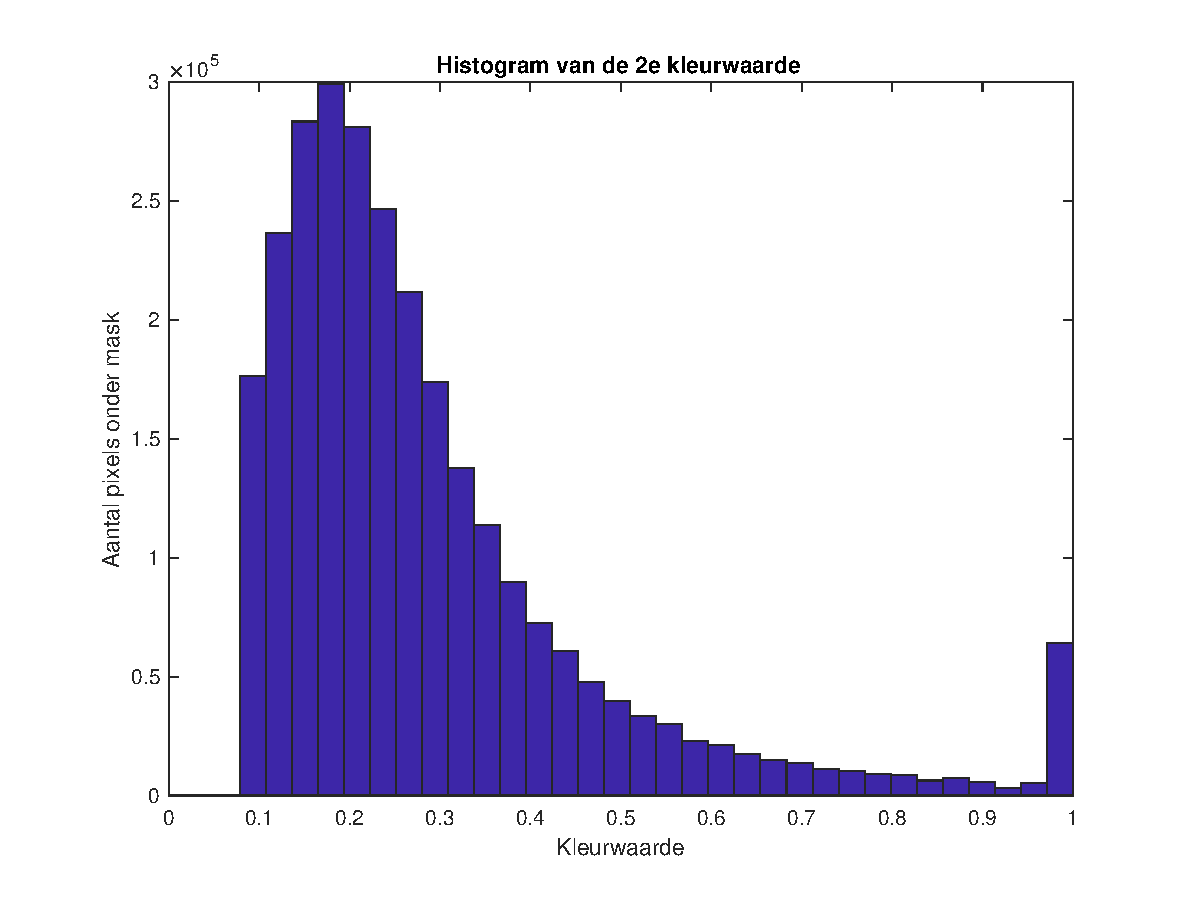
\includegraphics[width=4.5cm]{hsvhist_s}}}
	\qquad
	\subfloat[]{{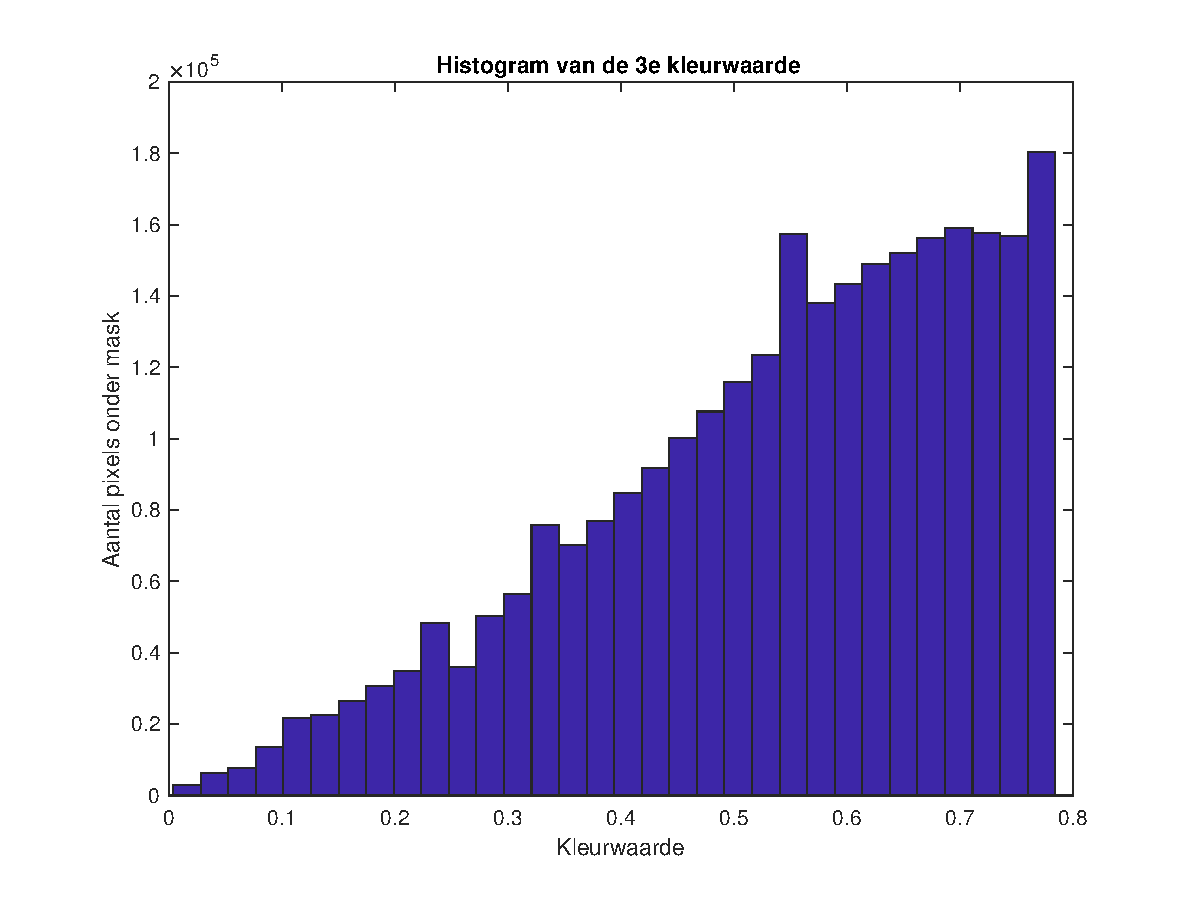
\includegraphics[width=4.5cm]{hsvhist_v}}}
	
	\caption{Histogrammen van de HSV kleurwaarden. We zien duidelijk het verschil in frequenties.}
	\label{figuur HSVHIST}
\end{figure}

\begin{figure}[H]
	\centering
	\subfloat[]{{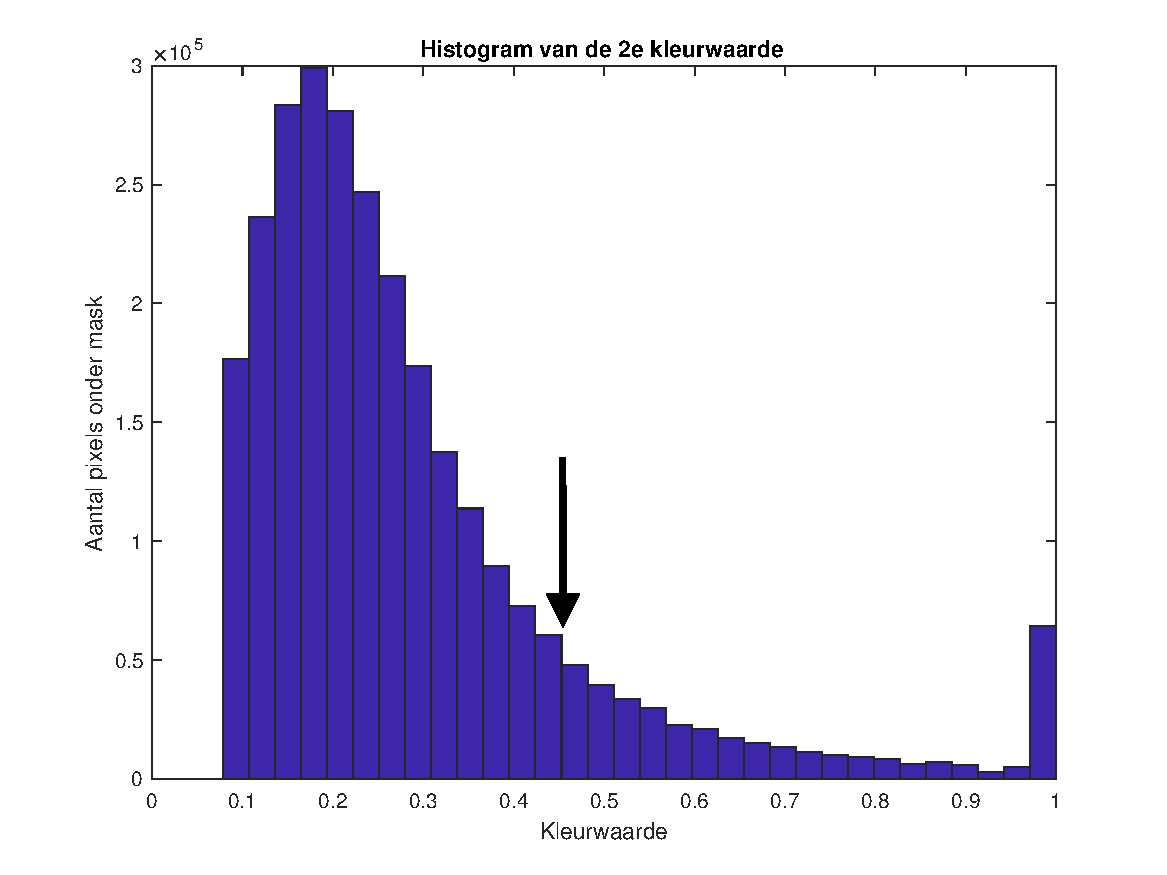
\includegraphics[width=0.7\textwidth]{hsvhist_aangeduid}}}
	
	\caption{Op de figuur is hebben we een punt op de curve aangeduid. Wanneer we dit punt naar links verschuiven, verwijderen we telkens grotere stukken indicator van onze afbeelding. Dit willen we net vermijden.}
	\label{figuur HSVHIST_aangeduid}
\end{figure}

\begin{figure}[H]
	\centering
	\subfloat[]{{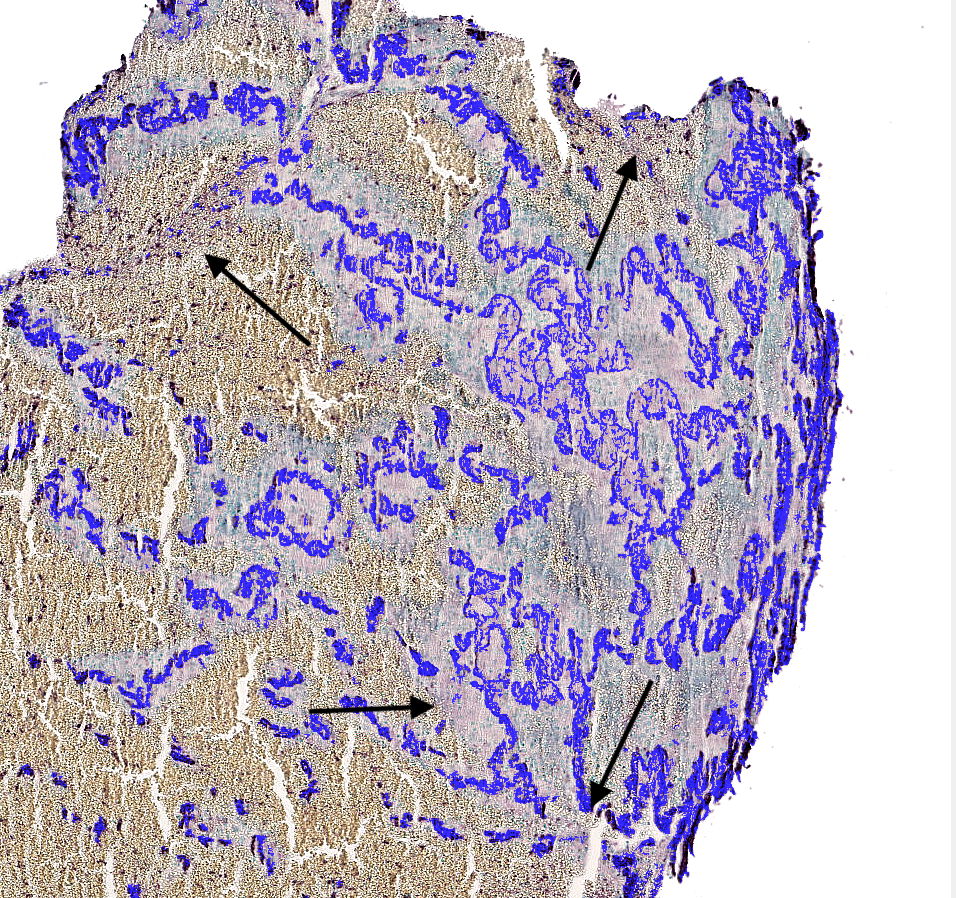
\includegraphics[width=7cm]{threshold_filtered}}}
	\qquad
	\subfloat[]{{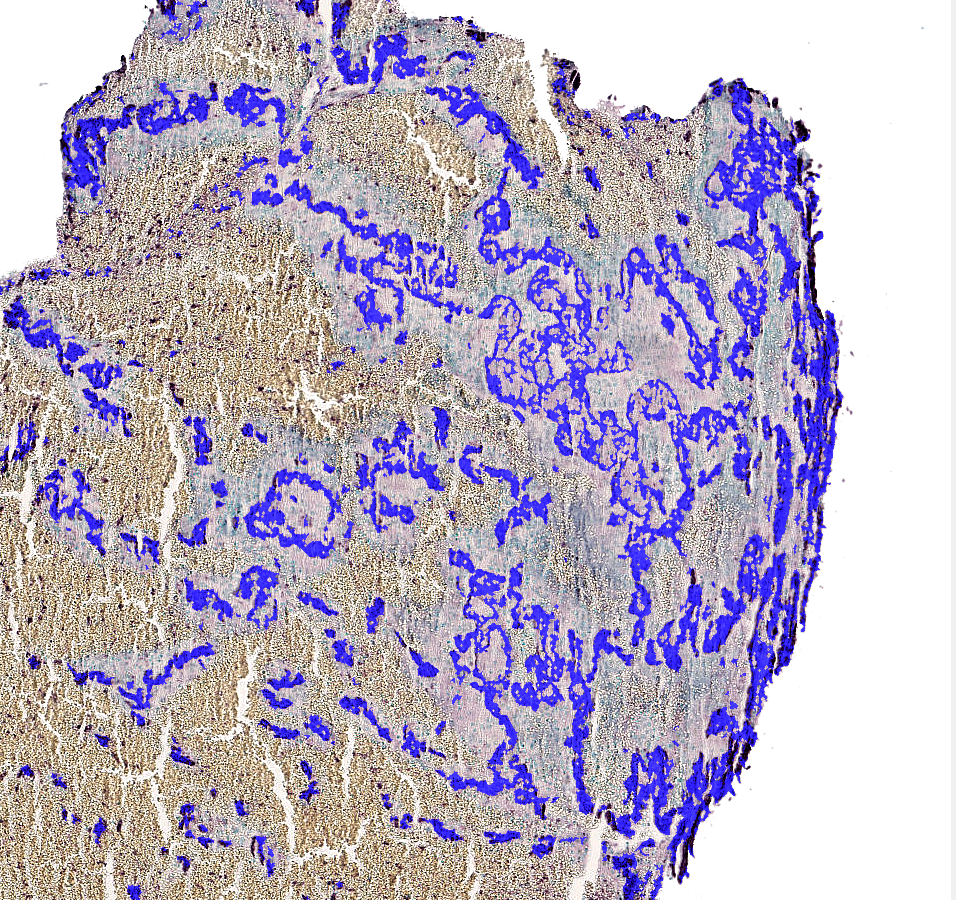
\includegraphics[width=7cm]{threshold_morfologisch}}}
	
	\caption{Illustratie waarbij we in (a) een algoritmische filter hebben toegepast om mogelijke ruis te verwijderen. De pijltjes zijn de zones die weggefilterd zijn op Figuur \ref{figuur alg_tresh}. In afbeelding (b) hebben we deze mask nog eens morfologisch gesloten, waardoor we een duidelijke aanduiding van de indicatorpixels bekomen.}
	\label{figuur morf}
\end{figure}

\subsubsection{Problemen}
De indicators worden nu wel met redelijke precisie in de afbeelding aangeduid, maar dit is niet even simpel voor elke afbeelding.
Het probleem met deze kleuringen is namelijk dat er heel wat variatie in de afbeeldingen zit. De effectieve kleuring in het labo is afhankelijk van verschillende factoren zoals bijvoorbeeld temperatuur, druk, luchtvochtigheid... Hierdoor kan deze kleuring van dag tot dag in intensiteit verschillen. Daarenboven zijn wij als student ingenieurswetenschappen ook niet getraind om rode bloedcellen te detecteren. Om hiervoor te compenseren zijn er in de app verschillende sliders om de filter bij te sturen. Zo kan toch altijd het gewenste resultaat bekomen worden.


\subsection{De gebruiksvriendelijke applicatie}
Naast het verwerken van de klonters is het ook de bedoeling dat de afbeelding op een makkelijke manier verwerkt kan worden. Vandaar dat we een gebruiksvriendelijke app in MATLAB gemaakt hebben. Aan de hand van MATLAB Coder is het mogelijk om een standalone versie van deze applicatie te creëren, waardoor de gebruiker geen MATLAB geïnstalleerd moet hebben. Een screenshot van de grafische interface van de app is te zien op Figuur \ref{figuur interface}. In dit hoofdstuk zullen we kort de functionaliteiten van deze app beschrijven.
De app kan op twee verschillende manieren gebruikt worden. In eerste instantie kan men een afbeelding ingeven die dan uiteindelijk het volledige verwerkingsproces van hoofdstuk \ref{Achtergrondverwijdering} en \ref{lokalisatie_indicator} doorloopt. Men begint met het kiezen van een afbeelding en een folder om de tussenresultaten op te slaan. In de eerste fase van het verwerkingsproces wordt de afbeelding bijgesneden zodat enkel de bloedklonter nog zichtbaar is. Deze bijgesneden afbeelding wordt dan getoond. Indien men niet blij is met de bekomen resultaten kan men manueel de threshold bijsturen. Vervolgens begint de kleurenanalyse, hier wordt de volledige afbeelding verwerkt om uiteindelijk een percentage indicator aan te duiden. Deze verwerkte afbeelding wordt dan ook getoond zoals te zien is op Figuur \ref{figuur interface}. Daarnaast wordt het percentage van de hoeveelheid aanwezige indicator weergegeven. Indien men niet tevreden is met het resultaat, kan men een transformatie naar een andere kleurruimte (HSV, CMYK of RGB) toepassen. Daarnaast kan men ook met verscheidene sliders een manuele selectie van de indicator doen. Men kan ten slotte nog opteren om de additionele filter uit hoofdstuk \ref{additional_filter} uit te schakelen. \\
De app kan ook op een andere manier gebruikt worden. Men kan namelijk een volledige folder met afbeeldingen selecteren om de achtergrond van iedere afbeelding te verwijderen. Deze afbeeldingen worden bijgevolg opgeslagen in een eerder gedefinieerde folder.

\begin{figure}[H]
	\centering
	\subfloat[]{{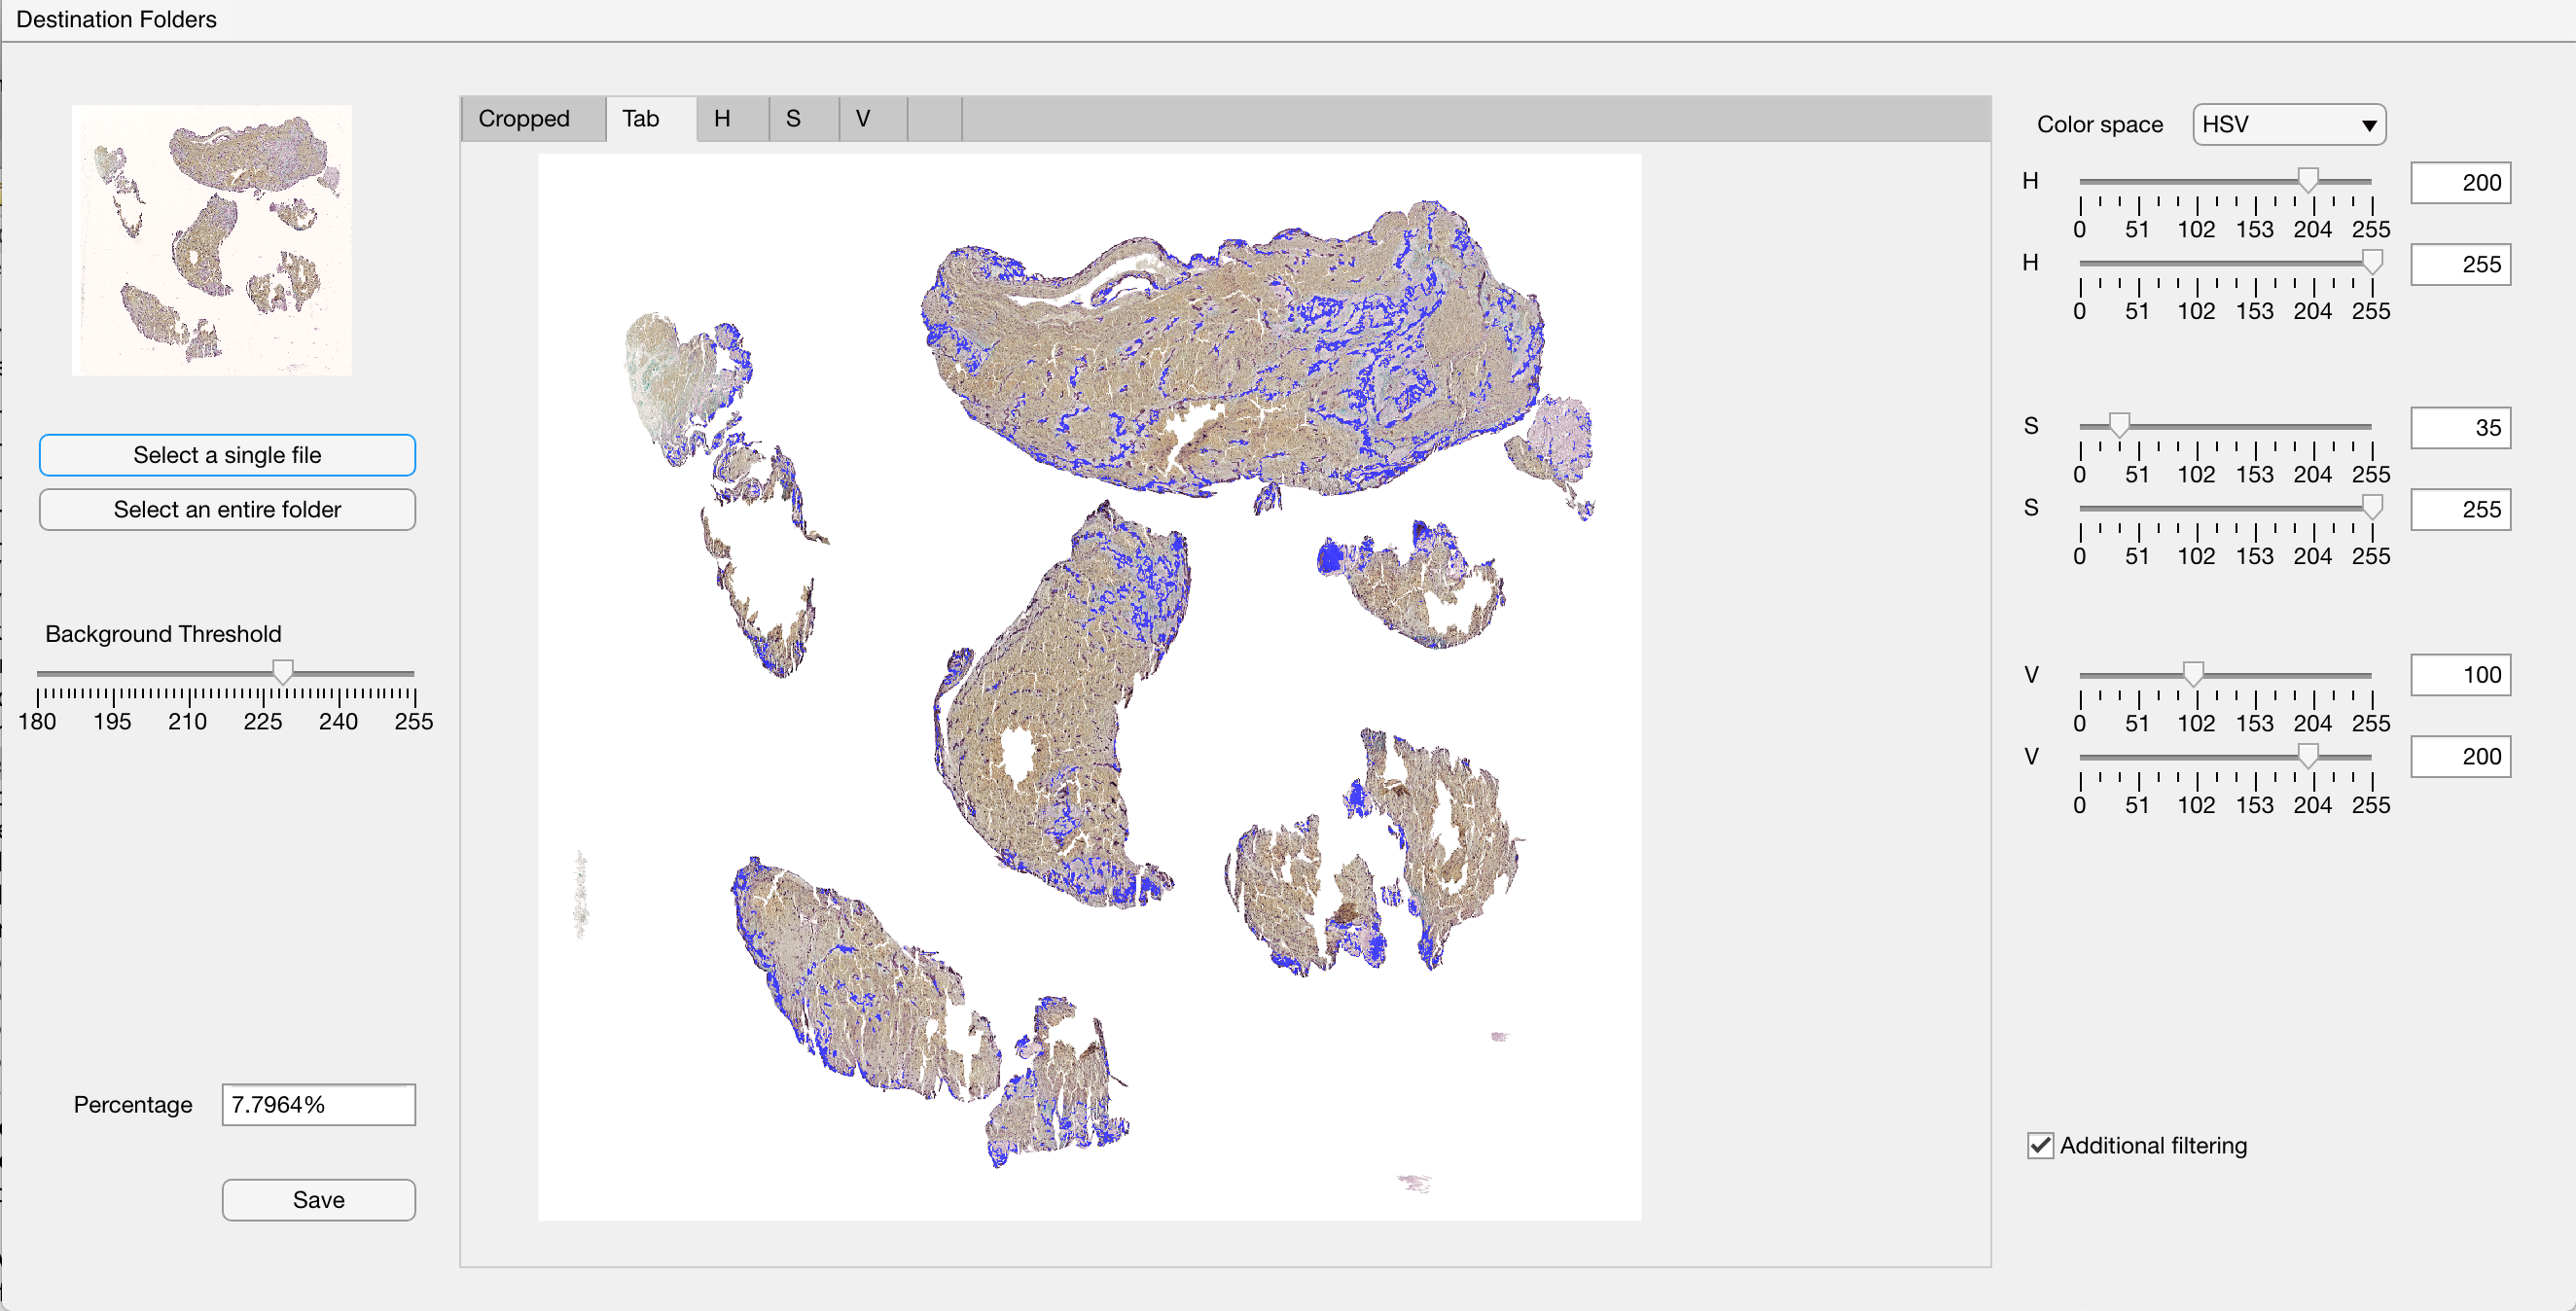
\includegraphics[width=\textwidth]{interface_app}}}
	
	\caption{Afbeelding van de grafische interface van de app.}
	\label{figuur interface}
\end{figure}

\section{Verantwoordelijkheden en taakverdeling}		
In onze groep hebben we ervoor gekozen om Robin aan te stellen als projectleider. Hij verdeelt elke week de taken en heeft het laatste woord bij discussies. 
Voor de verslagen en de eindpresentatie is Marthe verantwoordelijk. Zij is de eindredactrice van alle verslagen. We schrijven deze uiteraard samen, maar het is haar taak ervoor te zorgen dat deze volledig en gestructureerd zijn en dat ze voor de deadline ingediend worden.\\
Voor de implementatie van de code zijn we elk verantwoordelijk voor ons eigen deel. Zo wordt het verwijderen van de ruis en het bijsnijden van de afbeelding door Toon geleid, de kleurdetectie door Robin en de implementatie van de app door Marthe.\\
Helemaal achteraan dit verslag voegden we ook een Gantt-chart toe. Hierin staan enkele belangrijke deadlines vermeld en onze planning. We hebben het project opgesplitst in vier verschillende taken die we elk ingepland hebben zoals afgebeeld. Ook de tijd die we rekenen voor het tussentijds - en het finaal verslag, zijn af te lezen in de chart.

\section{Integratie van vakken}
Om dit probleem op te lossen, hebben we gebruik gemaakt van MATLAB. Het is dan ook een meerwaarde dat we in het eerste semester het vak 'Beginselen van Programmeren' gehad hebben om sneller vertrouwd te raken met deze nieuwe programmeertaal. Daarnaast leren we ook in 'nummerieke wiskunde' werken met MATLAB. Om de verschillende thresholds te bepalen in ons programma, maken we ook gebruik van en statistische analyse van de pixelwaarden. Het vak 'Statistiek' draagt hier dus ook zijn steentje bij.

\section{Besluit}	
We zijn erin geslaagd een app te ontwikkelen die de achtergrond op een afbeelding van een bloedklonter kan verwijderen. Daarenboven wordt de ruisvrije afbeelding automatisch bijgesneden. Ten slotte is er de mogelijkheid om het percentage van de hoeveelheid aanwezige indicator in de bloedklonter op te vragen.\\ 
De indicatoren worden in deze afbeelding vrij precies aangeduid maar dit is niet voor elke afbeelding even voor de hand liggend. Het is te wijten aan de onderlinge verschillen tussen de afbeelding door onder andere de kleuring die van intensiteit kan variëren. Daarom kan men manueel ingrijpen door middel van verschillende sliders. \\ 
Verder hebben we er rekening mee gehouden dat onze app gebruikt kan worden door klanten die geen MATLAB geïnstalleerd hebben. Dit zorgt ervoor dat ons eindresultaat voor iedereen gebruiksvriendelijk is.

\newpage
\bibliography{TTverslagbib}
\bibliographystyle{unsrt}

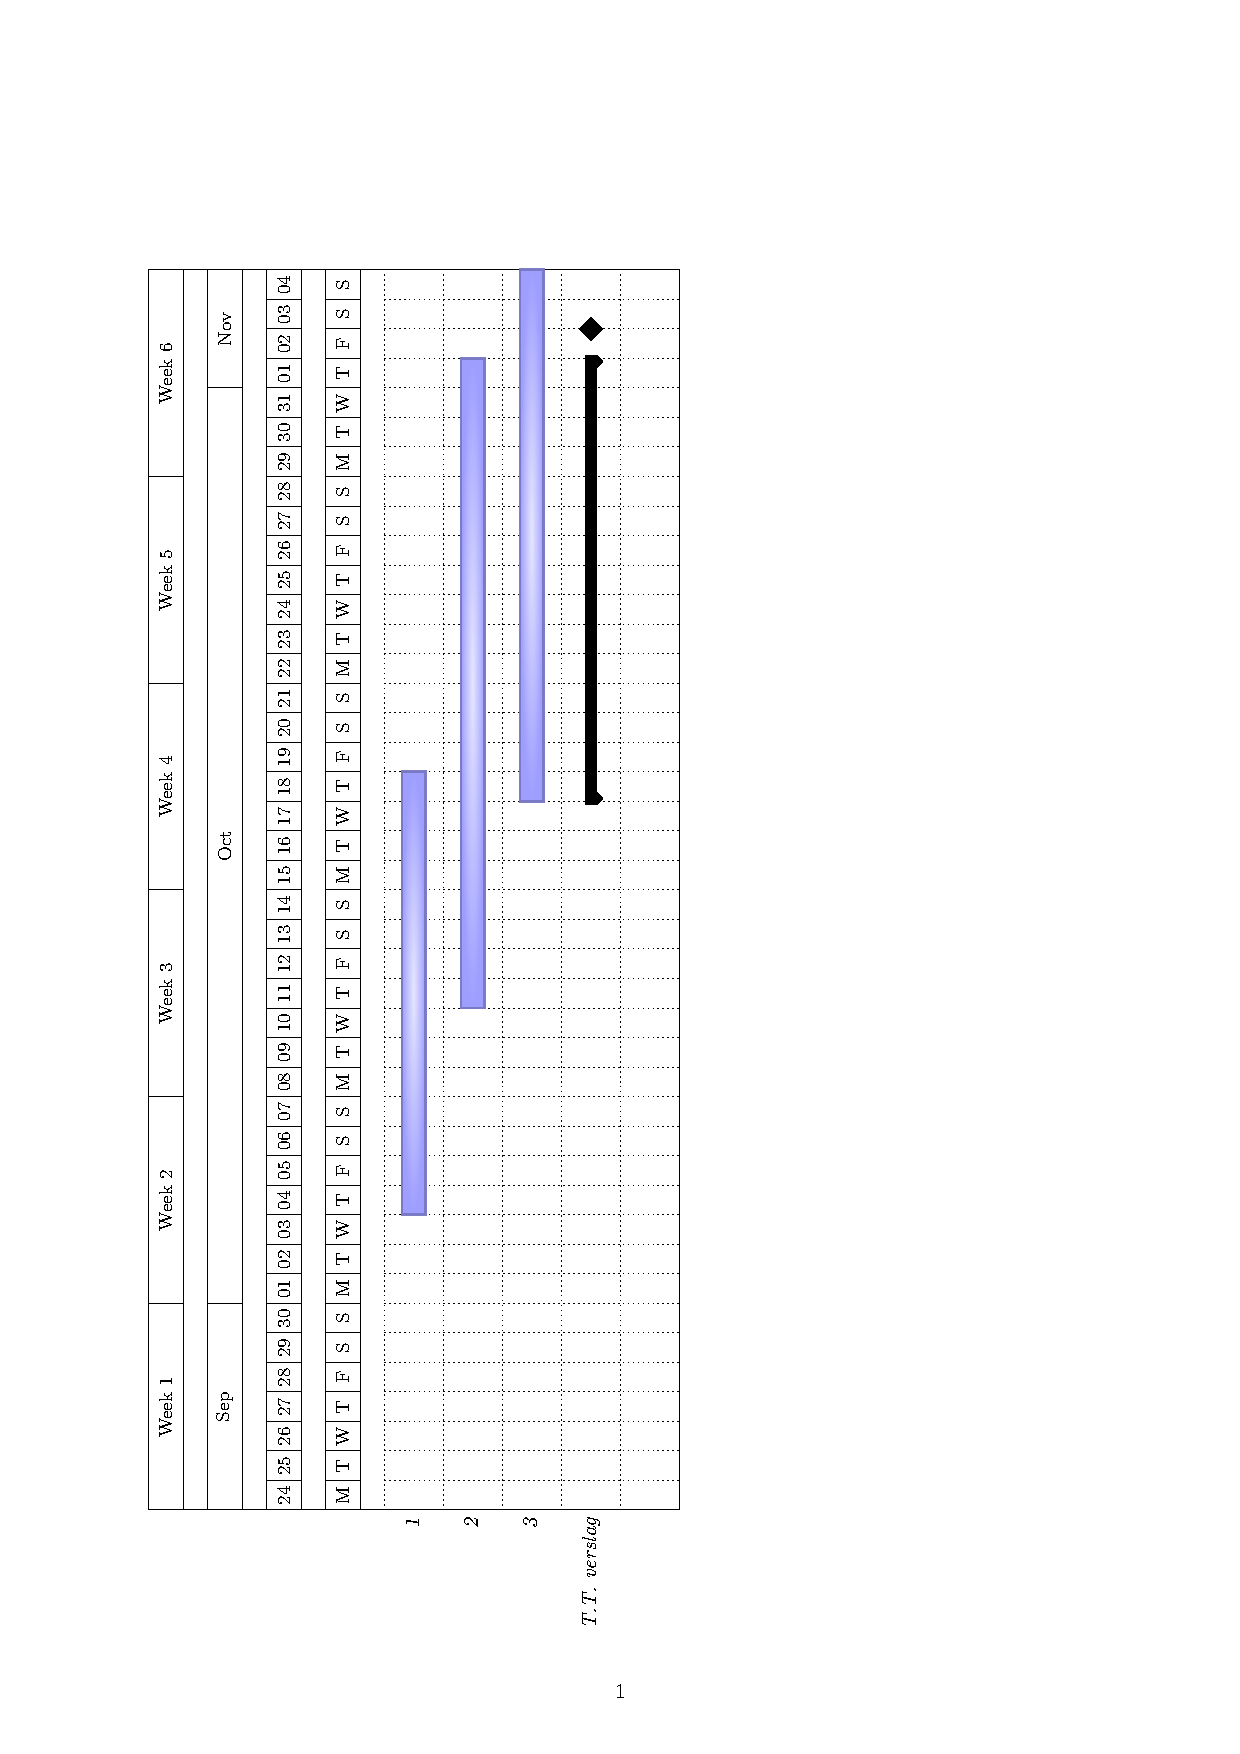
\includepdf[pages={1-3}]{ganttchart}

\end{document}
